\chapter{盆腔}

\section{检查方法}

\subsection{检查前准备}

1.胃肠道准备:空腹状态下,于检查前2~3小时左右分次口服2%泛影葡胺1000ml。必要时对直肠和乙状结肠于清洁灌肠后注入2%泛影葡胺或生理盐水150~300ml。

2.膀胱准备:①排泄法:CT检查前静脉注射泛影葡胺20ml;或让患者饮水,由尿液自然充盈。②逆行注入法:用Foley导管放尽尿液,注入2%~3%的泛影葡胺150~300ml,小儿酌减;亦可注入100~300ml气体和100ml泛影葡胺作双重对比CT检查。

3.其他准备:女性病人应常规放置阴道塞。

\subsection{CT扫描方法}

1.平扫:①常规仰卧位,从耻骨联合下缘扫描至髂嵴水平。特殊病例如发现盆腔内及腹膜后淋巴结转移、隐睾患者盆腔内未发现者等情况,扫描范围可扩至肾门水平或以上。②常规应用10mm层厚和间隔,发现小病灶后可3~5mm薄层扫描。③以软组织窗宽、窗位观察图像,特殊情况加骨窗或窄窗。④必要时可行冠状或矢状面扫描或重建。

2.增强扫描:经肘静脉以2~3ml/s的流率注入60%碘造影剂80~100ml。扫描方法同平扫。

\section{正常解剖和CT表现}

\subsection{精囊}

1.位置:位于膀胱后方、紧贴前列腺的上缘、直肠的腹侧。儿童期全部被腹膜覆盖,成人除外侧尖端外几乎全部在腹膜外。精囊与水平面交角约50°~60°,输精管行经其内侧缘,输尿管位于其前方,膀胱、前列腺静脉丛位于其外侧。精囊背缘以盆膈上筋膜与直肠相分隔。

2.形态:呈双侧对称性卵圆形软组织密度影。

3.大小:在CT图像上双侧共长6cm(亦有文献为7~8cm),在中线处两侧精囊汇合。

4.膀胱精囊角:精囊前缘与膀胱之间形成三角形脂肪间隙,称为膀胱精囊角或膀胱精囊三角(亦有文献称为精囊三角)。该角仰卧位时清楚;俯卧位时由于精囊前移贴近膀胱,可能消失。

\subsection{前列腺}

1.位置:紧贴膀胱尿道开口(膀胱颈)下缘、耻骨联合后方。其后缘由直肠膀胱筋膜相分隔,下缘与支撑盆腔脏器的尿生殖膈紧贴。

2.形态:其大体形态呈尖端向下的栗子形或圆锥形。CT图像上呈圆形、卵圆形密度均匀的软组织影,边缘清晰锐利。

3.大小:30岁左右,上下径平均约30mm,前后径约23mm,左右径约31mm;60~70岁则分别约50mm、43mm和48mm。

4.分叶和分区:由前叶、后叶、中叶和两个侧叶组成。成人除两侧叶外,其他3叶都很小(图\ref{fig21-1})。前叶很小,位于尿道前方;中叶呈上宽下尖的楔形,位于尿道后方,射精管之前;后叶位于射精管的后下方;两个侧叶紧贴尿道的侧壁,在后叶的前面。前列腺由腺体组织和非腺体组织构成,腺体组织主要分为3个区,即周边带(约70%)、中央带(约25%)和移行带(约5%)。

\begin{figure}[!htbp]
 \centering
 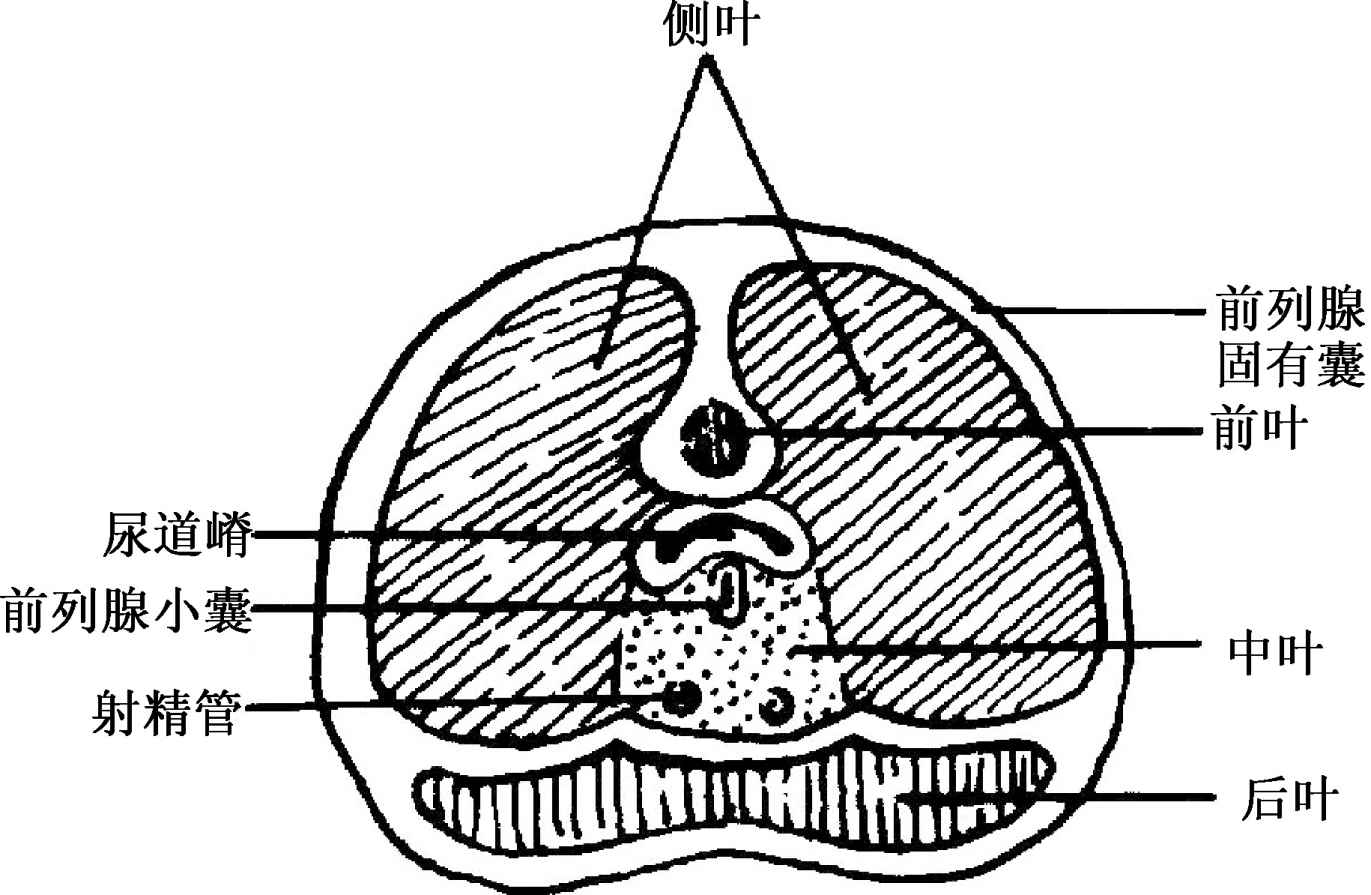
\includegraphics[width=.7\textwidth,height=\textheight,keepaspectratio]{./images/Image00397.jpg}
 \captionsetup{justification=centering}
 \caption{前列腺的横断面解剖}
 \label{fig21-1}
  \end{figure} 

\subsection{睾丸和阴囊}

1.位置:睾丸位于阴囊内,从外到里睾丸的被膜有阴囊皮肤、肉膜、提睾筋膜、提睾肌、睾丸精索鞘膜、睾丸固有鞘膜及白膜。两个睾丸通常不在一个高度,往往左侧低于右侧。

2.大小:睾丸上下径3~4cm,左右径1~2cm,前后径2~3cm。

3.CT表现:①阴囊壁:阴囊皮肤较松弛,带有小皱襞,密度较高;其下为密度较低的肉膜,厚度<1mm;肉膜至中线向深部形成阴囊隔。②睾丸:呈密度均匀的卵圆形软组织密度影;其四周由白膜包裹,呈细白轮廓线。当睾丸紧贴阴囊壁时,阴囊皮肤、肉膜、鞘膜及白膜呈现一条白线,难以区分。③鞘膜腔:一般显影不明显,正常含少量液体(0.5ml),如液体量增加称为鞘膜腔积液。

睾丸与附睾密度差异小,在CT上难以区分。

\subsection{子宫和卵巢}

1.子宫:①位置:膀胱位于子宫和阴道上段的前缘,前屈子宫紧贴膀胱后上缘,后屈子宫突入子宫直肠陷窝。②形态:分为底、体、颈3部分。在阴道上方CT层面上,子宫略呈圆形,横径约3~5cm;再上层面略呈纺锤形或三角形,位置可偏前、偏后或偏于一侧。子宫体中央密度略低。阔韧带由子宫侧缘伸延至盆腔内侧壁。③大小:在婴儿期宫体的大小与宫颈之比为1∶2;成年后则为2∶1。成年的子宫长(自宫颈至宫底)约7~9cm,左右径4~5cm,厚3~4cm。产后子宫可略大,绝经后子宫萎缩变小。

生育期妇女如子宫内膜厚度>10mm、绝经后如>5mm,为子宫内膜增厚。子宫体前后径>50mm为增大。

2.卵巢:位于子宫的两旁、阔韧带的后下缘,大小约4cm×2cm×2cm。输卵管在子宫上缘两侧,长约10cm。卵巢和输卵管通常不能被CT显示。

\subsection{盆腔壁侧和脏侧淋巴结}

盆腔淋巴结分为壁侧和脏侧。前者多位于盆壁内面,沿盆部血管排列;后者沿盆腔脏器分布。

1.盆腔壁侧淋巴结:①髂总动脉淋巴结:位于髂总动脉周围,每侧2~6个,又可根据与髂总动脉的关系分为髂总外侧、内侧和髂总中间淋巴结。②髂外淋巴结:沿髂外动、静脉排列,有3~10个,分为外侧、内侧和中间3群。③髂内淋巴结:沿髂内动脉干及其壁支排列,它包括闭孔、臀上和臀下淋巴结。在CT图像上一般位于骶髂关节下前方及闭孔内肌附近。④髂间淋巴结:位于髂内、外动脉起始部所形成的夹角内。⑤主动脉分叉下淋巴结:位于腹主动脉分叉的下方,相当于L\textsubscript{5}
椎体及骶骨岬的前面。

2.盆腔脏侧淋巴结:①膀胱旁淋巴结:位于膀胱的侧面及前面,其输出管注入髂内及髂间淋巴结。②阴道旁淋巴结:位于阴道上部侧方的结缔组织内,接受阴道上部及宫颈的集合淋巴管,其输出管注入髂间淋巴结。③直肠旁淋巴结:位于直肠壶腹部的后部及两侧,一般直径小于8mm,接受壶腹部的集合淋巴管,其输出淋巴管注入肠系膜淋巴结。

\subsection{男性盆腔的CT表现}

1.耻骨联合下缘层面:①在两侧耻骨前皮下脂肪中,可见密度不均的圆形软组织影为精索。其外方可见股静脉、股动脉及腹股沟浅淋巴结,正常淋巴结直径<1cm。②盆腔中线前方为前列腺,后方为直肠。前列腺呈椭圆形,正中为尿道,但尿道不能显示。③直肠不扩张时呈圆形软组织影,与周围脂肪界限清晰,外侧有提肛肌等组成条索状软组织影,或称直肠周围筋膜,其外后方为脂肪。④在此层面,盆腔外界为闭孔内肌。

2.耻骨联合上缘层面:盆腔中线内从前往后为膀胱、前列腺和直肠。两外侧界仍为闭孔内肌。

3.耻骨联合上方3cm层面:①充盈膀胱略呈长方形,壁厚<3mm。②膀胱后方为精囊,膀胱精囊角为锐角。③在两侧精囊外方,可见小点状软组织影,为膀胱静脉丛。④精囊以脂肪间隙与后方的直肠为界,直肠周围脂肪组织内可见小点状软组织影,为直肠静脉丛。⑤盆腔两侧界为闭孔内肌。

4.耻骨联合上方5cm层面:①盆腔前界为腹直肌,后方为骶骨。②两侧从前向后为髂外血管、闭孔内肌、梨状肌所构成。③坐骨神经位于梨状肌前方,CT上呈软组织密度影。

\subsection{女性盆腔的CT表现}

1.耻骨联合层面:①阴道由于填充阴道塞而呈圆形气影,其外周为阴道壁,壁外方有斑点状的阴道静脉丛。②阴道前方为膀胱,后方为直肠。

2.耻骨联合上3cm层面:①可见阴道塞影或宫颈的软组织影。②宫颈旁可见斑点状子宫静脉丛。③宫颈与盆腔侧壁的闭孔内肌或梨状肌之间有清晰的脂肪间隙,宫颈与后方的直肠间亦有脂肪间隙。④宫颈或阴道前方可为充盈的膀胱或小肠。

3.耻骨联合上5cm层面:①中央为子宫,呈横置的纺锤形,偶于两侧见阔韧带伸向前外方。②宫旁两侧脂肪中有斑点状的输尿管及子宫静脉丛。③子宫与直肠间、直肠与骶骨间有脂肪相分隔。④子宫两旁有时可见卵巢影,两侧大小可不对称,但与无造影剂的肠管不易区分。

4.耻骨联合上7cm层面:子宫呈三角形。在两侧梨状肌前内方,可见斑点状的髂内血管及细小淋巴结,正常淋巴结直径<1cm。子宫后方为乙状结肠。

\section{前列腺、精囊及睾丸病变}

\subsection{前列腺炎症和脓肿}

正常男性尿道远端5cm范围内及尿道黏膜下腺体内均有散在的病原体存在。正常的前列腺液中可有革兰氏阴性和阳性菌。前列腺外周区腺管开口于邻近膜部尿道处。腺管与后尿道呈直角关系,分泌物不易排出,尿道内细菌易进入腺体。而且因前列腺管长而弯曲、开口小,如有炎症或纤维化易致分泌物滞留,引起感染,故前列腺炎易发生于外周区。根据病因可分为细菌性和非细菌性。细菌性前列腺炎约95%是由革兰氏阴性杆菌引起的,常伴精囊炎。

\textbf{【病因病理】}
由于上述的解剖生理特殊所在,若饮酒过渡、纵欲或不正常性交、受寒、骑车、骑马等引起前列腺充血,是潜在的病原体繁殖而诱发前列腺炎。病原体可通过直接蔓延、血行和淋巴等途径而感染,尤以直接蔓延最常见。

急性者革兰氏阴性杆菌为最常见的致病菌,感冒和其他病毒也可诱发急性前列腺炎。慢性者可由急性前列腺炎迁延而来,但多无急性过程;常见致病菌为大肠杆菌、变形杆菌、葡萄球菌和链球菌等,还可见真菌、病毒、滴虫、支原体等致病;对原因不明的病例,称为慢性非细菌性前列腺炎或前列腺病态。

病理上急性者病变范围可为局限性或弥漫性。腺体有充血水肿及浆液纤维素性、血性和脓性渗出,以及炎性细胞浸润。严重者可形成单发或多发脓肿。慢性者渗出较少,呈慢性炎症改变;腺体也可因纤维性变而缩小、变硬即发生前列腺纤维化。

\textbf{【临床表现】}
急性者起病急,可有寒颤、发热、会阴部疼痛、排便或射精后疼痛,尿道有分泌物,尿流变细、尿频、尿急或尿潴留等。肛诊压痛明显,体积增大、光滑规则、质地柔软。一般临床即可诊断,勿需影像学检查,影像学以B超为首选。

慢性前列腺炎轻者可无症状。有症状者常为晨起时尿道外口被分泌物黏合,排尿不适或烧灼感、尿痛、尿频、尿急,会阴部不适,性功能障碍,腰骶部、睾丸或小腹胀痛。肛诊前列腺可大可小、表面不规则,部分变硬或有小结节。

\textbf{【CT表现】}

1.急性前列腺炎症和脓肿:常见体积增大,密度略减低(20~30Hu),边缘光滑。有液化坏死即脓肿形成时可有更低密度灶存在,增强扫描脓肿呈环状边缘强化。常伴精囊炎而表现为双侧精囊对称性肿大,密度减低;当排泄管不畅时,可单侧精囊增大或形成潴留性精囊囊肿。

2.慢性前列腺炎:有时在形态上难与前列腺良性增生鉴别,但也可因前列腺纤维化而表现为前列腺体积缩小。同样,慢性精囊腺炎亦可表现为对称性体积缩小。当然,前列腺纤维化也可为老年性退行性变所致,但影像学与感染所致者难以鉴别。

\subsection{前列腺结核}

\textbf{【病因病理】}
本病多继发于肾结核和其他泌尿生殖系结核,其中多继发于泌尿系结核。肾脏病变愈严重则合并男性生殖系统结核的几率越大。继发于尿路的结核,首先侵犯前列腺或精囊,然后沿输精管到达阴囊及睾丸。前列腺内形成结核病灶者,其体积增大、形态不规则;病情进展可出现坏死、干酪样变及钙化等病理改变。

\textbf{【临床表现】}
前列腺结核早期多无症状,严重者可出现会阴部坠胀不适、尿频、尿急、尿痛、尿混浊等慢性前列腺炎的表现。肛诊早期可正常,严重者腺体肿大呈不规则结节状,亦可呈坚硬肿块。可形成冷脓肿,甚至向周围溃破。

\textbf{【CT表现】}
无特异性,依其不同时期的病理变化而不同。典型者表现为前列腺体积略大或缩小,边缘凹凸不平,其内常见多个大小不等的不规则低密度坏死区,且常伴有斑点状钙化。增强扫描前列腺呈不均匀强化。

如无钙化存在,需与其他化脓性感染鉴别,有时需组织活检确诊。

\subsection{前列腺结石或钙化}

本病可发生于发育成熟男性的任何年龄组,但以40~70岁多见。

\textbf{【病因病理】}
病因不明,其发生可能与前列腺分泌液中淀粉样小体有关,这种小体由核蛋白、少量脂肪和晶体嘌呤包围脱落上皮细胞形成,在成人可随年龄的增长而增多。在前列腺有炎症或其他病理情况下,常以淀粉样小体、细菌团、血凝块或坏死组织为核心,发生钙化而形成结石。

本病可分为两类:①原发性:发生于前列腺的腺泡和导管。一般多发、细小,大小约1~5mm。可通过前列腺管排入尿道,常无症状。②继发性:常与感染、阻塞有关,钙化表示以往有炎症和梗死的病理过程,以后由于纤维化和钙盐沉积而形成,有时亦可见于放疗后。结石可伴癌瘤而发生,但与癌无因果关系。

\textbf{【临床表现】}
多数患者无特殊症状。但可有尿频、排尿困难,腰骶、会阴或阴茎部疼痛。如继发感染可出现寒颤、发热等全身症状。也可引起性功能障碍,如阳萎、早泄、射精时疼痛或血精等。

\textbf{【CT表现】}
无论原发性还是继发性,结石或钙化常为CT扫描偶然发现。多呈点状或圆形,亦可表现为较大的块状,边缘不规则,但一般<5mm(图\ref{fig21-2})。

\begin{figure}[!htbp]
 \centering
 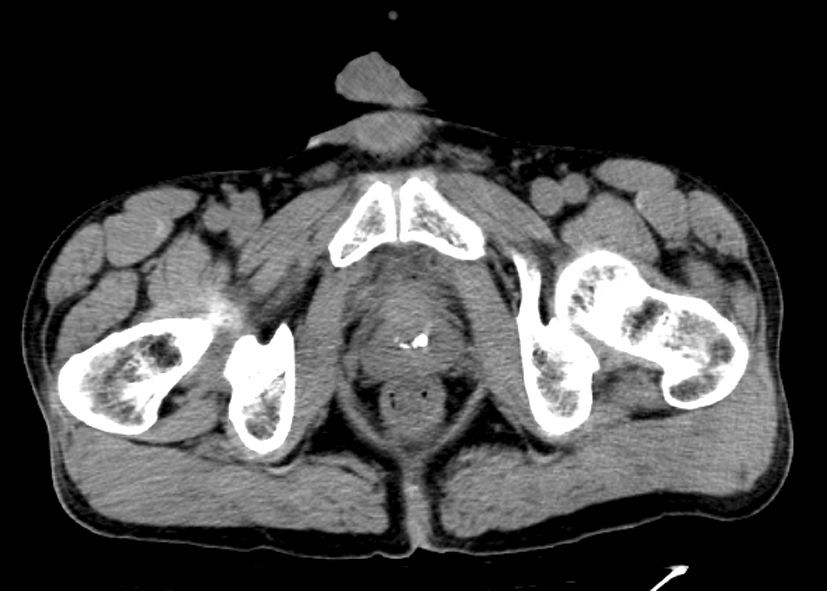
\includegraphics[width=.7\textwidth,height=\textheight,keepaspectratio]{./images/Image00398.jpg}
 \captionsetup{justification=centering}
 \caption{前列腺结石\\{\small 前列腺内有多个沙粒状高密度灶}}
 \label{fig21-2}
  \end{figure} 

\subsection{前列腺增生症}

本病是老年男性的常见病之一。40岁以前很少发生,50岁以后发病率约50%,60岁以上为60%~75%,而80岁后高达85%以上。

\textbf{【病因病理】}
其增生的原因较复杂,多认为与人体雄性激素与雌性激素的平衡失调有关。本病起源于中央区及移行区,尤其是后尿道旁区的腺组织、结缔组织及平滑肌组织。这些组织逐渐增生而形成多发性球状结节,真正的前列腺组织受到挤压,并推向外周而形成假性包膜。增生的组织很少发生癌变。

国内有学者报道根据病理和CT表现,前列腺体积偏大者以腺体或(和)平滑肌增生为主,体积不大者以纤维组织增生为主,密度不均为扩大囊变的腺体所致。CT强化部分为增生的前列腺中央区,不强化部分为萎缩的周边区,其中部分皱缩呈锯齿状。

\textbf{【临床表现】}
主要表现为尿频、尿急、夜尿、排尿困难。尿频为早期症状,后出现排尿困难、残留尿,甚至尿潴留。临床表现有时与腺体大小不成正比。可出现血尿,合并结石时更易出现终末血尿和排尿疼痛。肛诊表面光滑、质地中等硬度且有弹性。本病可并发膀胱憩室、精囊病变、尿道扩张及肾盂积水。

\textbf{【CT表现】}
正常前列腺上界不超过耻骨联合上缘10mm。当前列腺超过耻骨联合上缘20mm或更高,或(和)左右径超过50mm,即可诊断为增大(图\ref{fig21-3})。通常显示前列腺呈球形或椭圆形扩大,两侧对称、边缘光滑、密度均匀,常有钙化。周围脂肪间隙清晰,膀胱精囊三角正常。增生前列腺常向上推挤膀胱底部形成“双叶”征象。有时明显突入膀胱,似膀胱内肿块,但膀胱壁均匀完整有助于鉴别。增强扫描前列腺的中央区围绕尿道周围或略偏一侧(即增生的区域)可有圆形明显强化区,而周边区无明显强化。

\begin{figure}[!htbp]
 \centering
 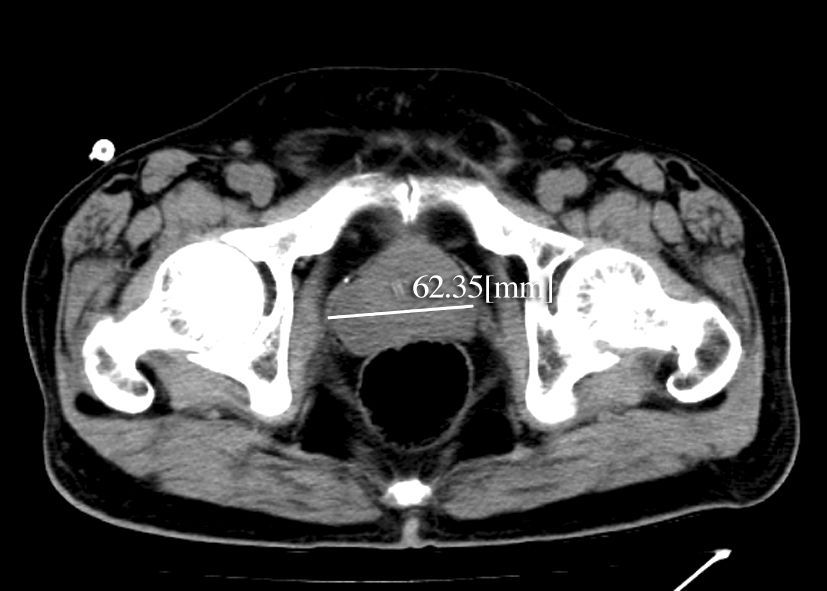
\includegraphics[width=.7\textwidth,height=\textheight,keepaspectratio]{./images/Image00399.jpg}
 \captionsetup{justification=centering}
 \caption{前列腺增生\\{\small 前列腺体积增大,密度较均匀}}
 \label{fig21-3}
  \end{figure} 

\subsection{前列腺囊肿}

\textbf{【病因病理】}
有先天和后天之分。①先天性前列腺囊肿:又称前列腺小囊。发生于中肾管或副中肾管系统残余部分的上皮,囊肿常位于前列腺上方、膀胱后面的正中线处,体积可很大。②后天性前列腺囊肿:主要指潴留性囊肿。囊壁为腺泡上皮,由立方或扁平上皮所覆盖。囊肿可位于任何部位,或突至膀胱颈部,直径多为1~2cm。囊液澄清,亦可为暗褐色或血色,囊液内可含精子。

\textbf{【临床表现】}
无特异性,可有尿急、尿频、排尿费力、尿流变细、残留尿及尿潴留。先天性常伴尿道下裂、阴睾、肾发育不全或不发育。

\textbf{【CT表现】}
前列腺内边缘清晰、光整的水样密度灶,CT值10Hu左右。病灶与周围正常腺体组织界限清晰。增强扫描无强化。

\subsection{前列腺癌}

本病为欧美男性癌症患者死亡的主要原因之一,我国发病率较低。

\textbf{【病理】}
95%以上为腺癌,其余为移行细胞癌、鳞癌和肉瘤。75%起源于后叶包膜下区,常累及侧叶,其次为移行区,少见于中央区。常为多病灶,常伴有增生。

转移途径:①局部转移:可侵犯尿道、膀胱颈和精囊,甚至输尿管膀胱入口,一般不侵及直肠。②淋巴转移:最常侵犯髂内、外等盆腔组和腹膜后淋巴结。③血行播散:以骨骼转移最多见,常见的部位为骨盆、腰椎、胸椎、肋骨等。实质脏器转移以肺、肝、肾上腺等多见。

\textbf{【临床表现】}
早期多无症状或出现前列腺增生相似的症状。晚期出现腰骶或髂部疼痛、膀胱区或阴茎疼痛、直肠或会阴部疼痛,并可有便秘、消瘦、乏力和进行性贫血。直肠指检常可触到前列腺硬结,质地坚硬、表面不规则。晚期血清酸性磷酸酶常升高。

\textbf{【CT表现】}
早期仅显示前列腺增大,而密度无异常改变;增强扫描肿瘤与前列腺强化类似,而无助于诊断局限于被膜内的肿瘤。

进展期诊断要点:平扫前列腺常呈不匀称增大或局限性向外突出(图\ref{fig21-4});癌灶密度多数低于正常前列腺组织(癌灶内可见钙化);增强扫描结节边缘多数清楚,但密度均较正常区域低。较早累及精囊、膀胱是其另一特征。此外,淋巴和血行转移表现有利于进一步确诊。

\begin{figure}[!htbp]
 \centering
 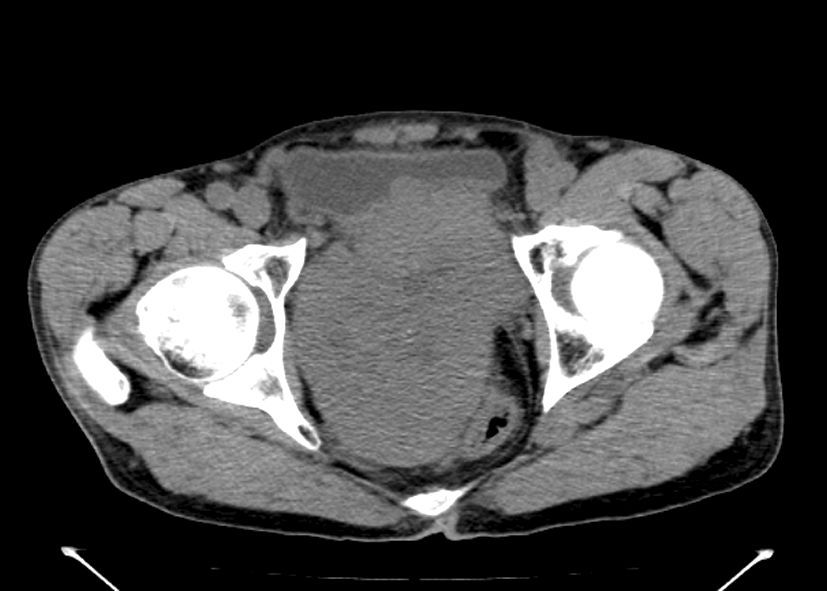
\includegraphics[width=.7\textwidth,height=\textheight,keepaspectratio]{./images/Image00400.jpg}
 \captionsetup{justification=centering}
 \caption{前列腺癌\\{\small 前列腺显著增大,密度不均,边缘不规则;膀胱和直肠显著受压(本例伴有髂内、外组淋巴结转移)}}
 \label{fig21-4}
  \end{figure} 

\textbf{【鉴别诊断】}

1.前列腺增生:①前列腺边缘尤其是后缘、外后缘结节状隆起和边缘毛糙,并见局限性密度减低是CT诊断前列腺癌的主要征象。若低密度位于前叶或中叶,伴有前列腺匀称性体积增大、边缘光整常为前列腺增生的表现。②前列腺增生前列腺的中央区有强化而周边无明显强化,有别于增强扫描呈低密度灶的前列腺癌。

2.膀胱癌侵犯前列腺:常以直接浸润的方式累及前列腺,但一般无前列腺增大,有时两者因果关系不易区分。

3.后尿道球部肿瘤:表现为紧贴前列腺的不规则肿物,大部突出于前列腺外,密度不均,靠膀胱尿道镜检确诊。

4.前列腺炎性肉芽肿:在前列腺增大基础上,内有不规则模糊低密度区,范围较大(占居约1/2),难与肿瘤鉴别。

5.前列腺结核:多与肾、附睾、膀胱结核并存。前列腺正常、增大或缩小,其内有低密度区伴钙化,轮廓欠清楚,需结合其他检查确诊。

6.前列腺囊肿、脓肿:①囊肿呈前列腺内一边缘清楚的薄壁囊状水样密度灶,可向外突出;②脓肿可呈多房、壁厚,边缘欠清,内容物为水样或脓液性物,与癌灶的不规则低密度、边缘模糊影有别。

7.前列腺良性肿瘤:可为实性、囊性(甚至多囊状)或囊实性密度灶,CT表现无特异性。

\subsection{精囊炎}

\textbf{【病因病理】}
多由细菌感染或寄生虫引起(结核性感染后述)。精囊炎由细菌经尿道上行蔓延、来自精路或血行感染。病原菌多为葡萄球菌、链球菌、大肠杆菌等。开始时精囊黏膜充血水肿,继而形成局部脓肿,甚至破至精囊周围。精囊感染时,常同时有前列腺炎或后尿道炎。

\textbf{【临床表现】}
急性精囊炎常有发热、寒颤等全身症状,局部可有下腹痛,并可延及腹股沟和会阴。常因后尿道受累而出现尿急、尿频、尿痛、排尿困难、血尿及尿道分泌物等症状,血精为其特征。慢性精囊炎与慢性前列腺炎不易区别,常同时存在,但慢性精囊炎有血精的特征。

\textbf{【CT表现】}
精囊体积增大,形态饱满,密度减低,CT值多为20Hu左右。增强扫描常见精囊呈不均匀强化,并可见条状显著强化及不规则无强化的水样密度区。

\subsection{精囊结核}

\textbf{【病因病理】}
男性生殖系结核多与泌尿系结核同时存在(50%~80%)。男性生殖系结核多继发于泌尿系结核,部分肺结核病灶血行播散时,肾和生殖系同时受累,也有少数仅有生殖系受累。男性生殖系统结核往往从前列腺、精囊开始,后蔓延到输精管、睾丸及附睾。病理显示精囊形态不规则,可出现坏死、干酪样变及钙化等病理改变。

\textbf{【临床表现】}
多无明显症状,常在附睾结核出现临床症状时,肛诊发现精囊硬结。患者可出现血精及精液量减少,病变波及输精管可导致不孕。

\textbf{【CT表现】}
精囊大小不等,可有低密度脓肿。典型表现为体积缩小、形态不规则,密度欠均匀,内有散在的钙化灶。增强扫描呈不均匀强化,其内有不规则的无强化的低密度坏死区。

\subsection{精囊结石}

\textbf{【病因病理】}
多由于精囊的慢性炎症、腺管黏膜粗糙,引起无机盐(如磷酸钙和碳酸钙)结晶附着在脱落的上皮细胞和炎性渗出物上而形成的。一般为棕色光滑的多发性小结石。

\textbf{【临床表现】}
腹股沟处疼痛,常延及睾丸和会阴。结石可嵌顿于射精管中阻碍精液的排出,引起如输尿管结石相似的疼痛,在有性冲动及射精时加剧,血精较常见。

\textbf{【CT表现】}
平扫示精囊内单个或多个斑点状高密度灶,大小一般为1~3mm,呈块状高密度灶者少见。

\subsection{精囊囊肿}

本病较为罕见。

\textbf{【病因】}
①先天性:由于射精管的先天闭锁,导致精囊全部或部分阻塞,形成单个或多个囊肿。国外有学者还认为与常染色体显性遗传的成人多囊肾有关。②后天性:可因多种原因造成的射精管阻塞,如炎症、膀胱颈部疾病或血精等。

\textbf{【临床表现】}
以20~40岁多见。较小者无症状,偶然发现。大者可出现下腹部的烧灼感、不适感或疼痛,排尿困难和尿频,如合并感染和结石可引起血精、血尿和不育症。

\textbf{【CT表现】}
典型者见精囊部单侧或双侧偏离中线且边缘规整的薄壁水样低密度灶,亦可呈边缘不规则的多囊腔。密度不均为囊内出血和结石所致,囊壁偶见钙化。大小不一,多<5cm,大者可达10cm以上。增强扫描无强化。

\textbf{【鉴别诊断】}
应注意排除罕见的精囊肿瘤,如平滑肌肉瘤有坏死囊变时可类似本病,但平滑肌肉瘤多界限不清。

\subsection{精囊肿瘤}

\textbf{【病因病理】}
精囊原发性肿瘤少见,多为继发性。原发精囊癌以来自上皮的乳头状瘤或癌占多数;间质的肉瘤来源于精囊的纤维肌肉组织。继发性的肿瘤多来自前列腺癌、膀胱癌及直肠癌的直接蔓延,也可继发于胃癌等在盆腔内的播散。

\textbf{【临床表现】}
精囊肿瘤尤其是精囊癌的早期症状为血精。肿瘤较大时可有尿频、尿急、血尿及排尿障碍,可有腹股沟区及睾丸的疼痛。晚期可有消瘦、乏力及直肠压迫所致的排尿困难。

\textbf{【CT表现】}
平扫示精囊不规则增大,形态不规整,密度不均,周围脂肪间隙消失。增强扫描呈不均匀强化,与周围正常组织界限不清晰。

\subsection{隐睾}

睾丸未下降至阴囊内通称为隐睾。

\textbf{【病理】}
可分为3类:①先天性无睾丸:约占3%~5%;②移行睾丸:约占70%,间歇性位于阴囊内,其退缩为提睾肌收缩所致;③真性睾丸下降不良:约占30%,睾丸可能位于接近腹外环的高位阴囊中,亦可在腹股沟内或超过腹内环位于腹内。隐睾可单侧或双侧发病,后者占10%;停留在腹膜后占25%,腹股沟70%,阴囊上部及其他部位占5%;50%~70%伴腹股沟斜疝。

病理上,隐睾较正常睾丸小而软,常并发附睾、睾丸连接处畸形。镜检尤其3岁以后可见隐睾曲精管退变,上皮细胞萎缩,致生育功能障碍。

\textbf{【临床表现】}
隐睾无症状,多因阴囊内无睾丸而就诊。常在腹股沟处触及小而活动的睾丸,多无内分泌障碍。

\textbf{【CT表现】}
①沿正常睾丸下降途径区,可见未下降睾丸呈软组织块影,圆形或卵圆形,边缘一般清楚。②当未下降睾丸特别大时,应疑有恶变(图\ref{fig21-5})。③萎缩的睾丸和邻近结构的鉴别有时困难。增强扫描有助于与血管相鉴别。

\begin{figure}[!htbp]
 \centering
 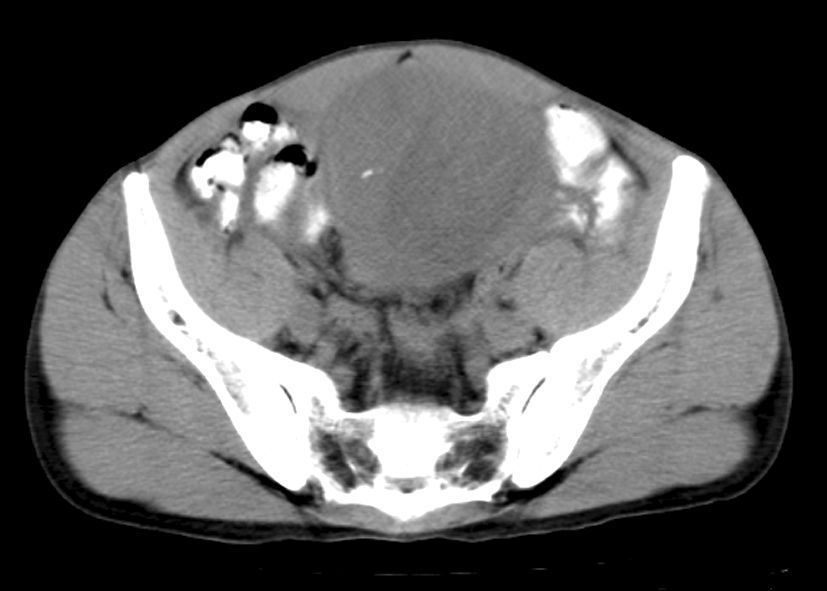
\includegraphics[width=.7\textwidth,height=\textheight,keepaspectratio]{./images/Image00401.jpg}
 \captionsetup{justification=centering}
 \caption{隐睾恶变\\{\small 双侧隐睾患者,盆腔内可见巨大软组织肿块,密度不均,其内有低密度坏死和高密度钙化表现,界限欠清晰,病理为精原细胞瘤}}
 \label{fig21-5}
  \end{figure} 

\subsection{睾丸炎}

\textbf{【病因病理】}
睾丸炎性病变可由各种致病菌引起,可分为非特异性、寄生性和自发性(找不出致病因素)等类型。常见的为非特异性睾丸炎和腮腺性睾丸炎。

非特异性睾丸炎病理表现为睾丸肿大,阴囊壁水肿,鞘膜脏层充血红肿,鞘膜腔内渗出液。局部坏死、白细胞浸润、曲精管上皮细胞破坏,有时整个睾丸化脓。慢性期鞘膜增厚、鞘膜腔闭锁,睾丸纤维化萎缩。腮腺炎性睾丸炎多为单侧(2/3),曲细精管有炎性细胞浸润。

\textbf{【临床表现】}
非特异性睾丸炎常有寒颤、发热,睾丸疼痛向腹股沟放射,可有恶心、呕吐,阴囊皮肤明显红肿且有压痛。腮腺炎性睾丸炎与非特异性睾丸炎类似,但病情较轻。

\textbf{【CT表现】}
睾丸密度尚均匀,密度较正常睾丸略低,部分可伴有鞘膜积液表现。如为肉芽肿性睾丸炎,睾丸呈不均匀性增大,边缘不整,密度不均,并可见小的坏死囊变区。

\subsection{睾丸结核}

\textbf{【病因病理】}
常由附睾结核直接蔓延而来,前列腺和精囊是生殖系结核的原发病灶,而附睾结核是生殖系结核的晚期表现。睾丸结核病理也为干酪样变、斑痕形成及钙化等,可并发鞘膜积液。

\textbf{【临床表现】}
除原发部位的症状和体征外,也可有局部的疼痛、阴囊皮肤红肿,常合并鞘膜积液或局部的脓肿,睾丸表面有结节感。

\textbf{【CT表现】}
睾丸普遍性增大或局部肿大,内部呈软组织密度,边缘可不清晰。如有脓肿形成及纤维增殖钙化时,内部密度不均,可显示斑点状高密度的钙化影。部分患者因睾丸鞘膜内积液而呈液性低密度。

\subsection{睾丸鞘膜腔积液}

\textbf{【病因病理】}
睾丸周围的鞘膜囊内存有过多的液体时称为鞘膜腔积液。其类型与鞘状突是否闭锁密切相关。其中以睾丸鞘膜积液最常见,其次为精索鞘膜积液、混合和交通性鞘膜积液,以及婴儿型鞘膜积液。

鞘膜积液的病因可分为原发性和继发性两种。前者多无明显的原因,起病缓慢,病理上常见鞘膜有炎症反应,可能与慢性创伤和炎症有关。小儿睾丸鞘膜的淋巴系统发育较晚,如睾丸与腹腔之间的鞘状突过早闭合,则鞘膜囊内的分泌液不能完全吸收,即形成先天性积液;当鞘膜的淋巴系统发育完善,积液可自行吸收。继发性鞘膜积液则有原发疾病,如急性睾丸炎、附睾炎、精索炎、创伤或疝修补、腹水、肿瘤等。

原发性积液呈清亮的淡黄色,如有出血呈棕色。炎症者为渗出液,严重时可呈脓性。鞘膜壁常有纤维化和钙化。慢性鞘膜积液可引起睾丸萎缩。

\textbf{【临床表现】}
一般无自觉症状。当大量积液时,张力高可有牵扯痛或下坠感。巨大者可影响排尿。继发性常有原发病的症状。

\textbf{【CT表现】}
睾丸侧方或(和)上方呈圆形、椭圆形或梨形囊状病灶,其内为水样密度(图\ref{fig21-6})。以固有鞘膜为主的囊壁厚薄均匀、规整光滑,病灶与睾丸关系密切。

\begin{figure}[!htbp]
 \centering
 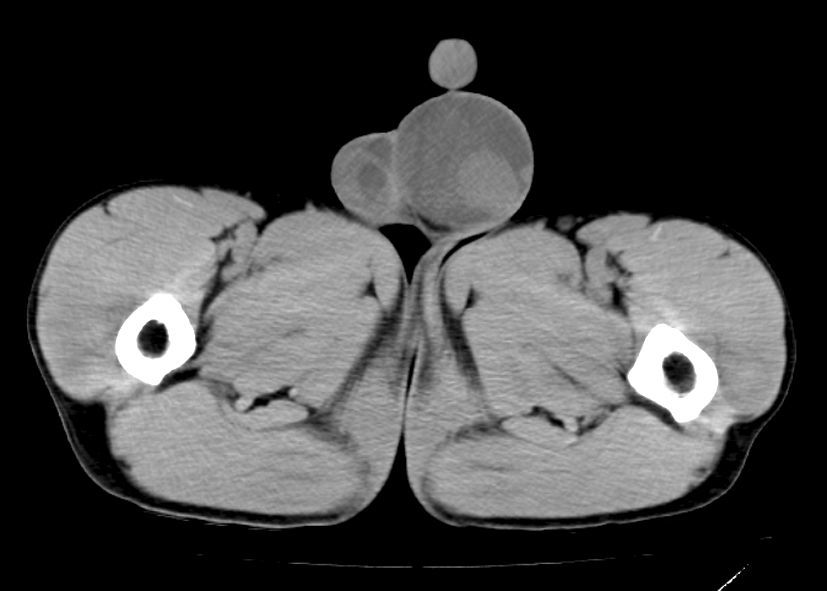
\includegraphics[width=.7\textwidth,height=\textheight,keepaspectratio]{./images/Image00402.jpg}
 \captionsetup{justification=centering}
 \caption{鞘膜腔积液\\{\small 左侧睾丸周围大量水样密度区}}
 \label{fig21-6}
  \end{figure} 

\subsection{睾丸肿瘤}

睾丸肿瘤在我国发病率较低,占男性全部肿瘤的1%~2%。

\textbf{【病因病理】}
一般多为原发性,继发性极为罕见。原发性绝大多数为恶性,可能与隐睾、外伤、炎症、内分泌及致癌物等有关。原发恶性肿瘤多起源于原始生殖细胞(90%~95%)。生殖细胞肿瘤中最常见的为精原细胞瘤(占40%~70%),其次为胚胎性癌(占全部睾丸肿瘤的20%),偶见绒膜上皮癌。良性肿瘤少见,约占睾丸原发性肿瘤的3%~4%,且多起源于非生殖细胞如纤维组织、平滑肌、横纹肌、血管和淋巴组织,但也有文献认为良性者多为成熟畸胎瘤。继发性通过血行、淋巴途径或直接蔓延而至睾丸。

\textbf{【临床表现】}
生殖细胞瘤绝大多数发生于50岁以前,其中精原细胞瘤多见于30~40岁;胚胎性癌和畸胎瘤多见于20~30岁。早期症状不明显,典型表现为逐渐增大的无痛性肿块。偶可有内分泌失调的症状,如男性乳腺发育、性早熟或女性化。肿瘤出血、坏死可出现急性疼痛,类似感染的表现。

\textbf{【CT表现】}
原发病灶表现为两侧睾丸大小不对称,患侧睾丸明显肿大且边缘不甚规则的软组织肿块(图\ref{fig21-7})。肿块密度多不均匀,其内可有不规则低密度坏死区,部分可见出血。增强扫描呈不均匀强化,但有时与来源于阴囊的肿瘤不易鉴别。

\begin{figure}[!htbp]
 \centering
 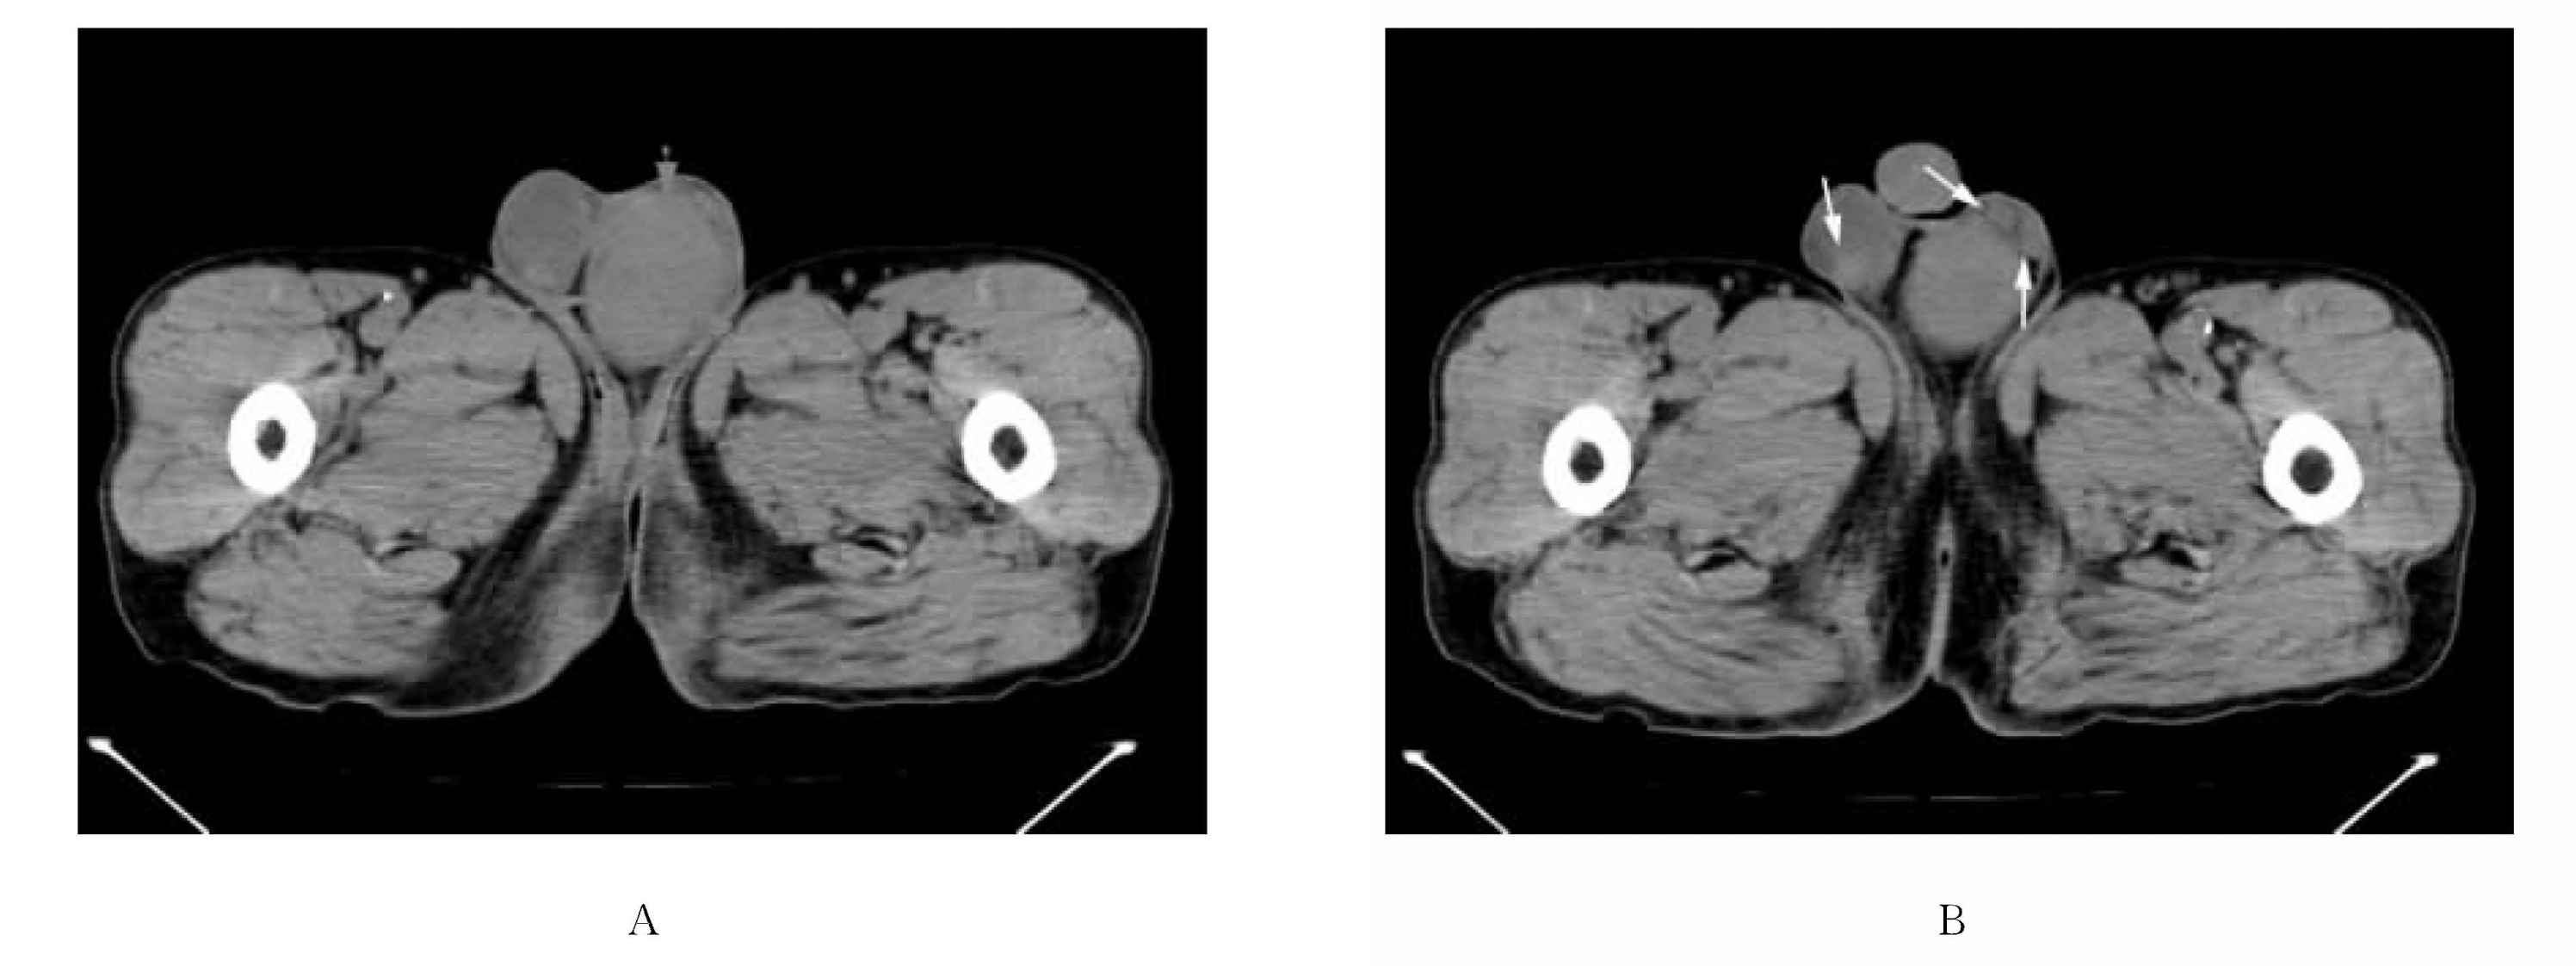
\includegraphics[width=.7\textwidth,height=\textheight,keepaspectratio]{./images/Image00403.jpg}
 \captionsetup{justification=centering}
 \caption{睾丸恶性淋巴瘤(NHL)\\{\small 患者70岁。A示左侧睾丸显著增大,密度较均匀;B示增大的左侧睾丸前方和右侧睾丸上方有高密度小结节}}
 \label{fig21-7}
  \end{figure} 

CT扫描的主要作用是对诊断明确的睾丸肿瘤患者,发现其盆腔、腹腔、纵隔的转移淋巴结以及实性脏器(肺、肝、肾等)的转移,以明确分期。

\subsection{阴囊内闭合性损伤}

\textbf{【病因病理】}
睾丸损伤的常见致伤原因多为直接暴力。损伤可分为闭合性和开放性两类;按损伤程度可分为睾丸挫伤、裂伤、脱位和扭转。睾丸损伤常伴有鞘膜积液、积血或阴囊血肿等。

\textbf{【临床表现】}
局部疼痛,可放射到下腹或腰部。重者可发生疼痛性休克。但有时疼痛不重,而以局部肿胀或阴囊血肿为主,可有恶心、呕吐。

\textbf{【CT表现】}
①阴囊肿大;②肉膜增厚模糊;③鞘膜腔积液(图\ref{fig21-8}A);④睾丸肿大;⑤实质内出血(图\ref{fig21-8}B);⑥睾丸白膜破裂;⑦白膜下血肿;⑧阴囊隔肿胀偏移。

\begin{figure}[!htbp]
 \centering
 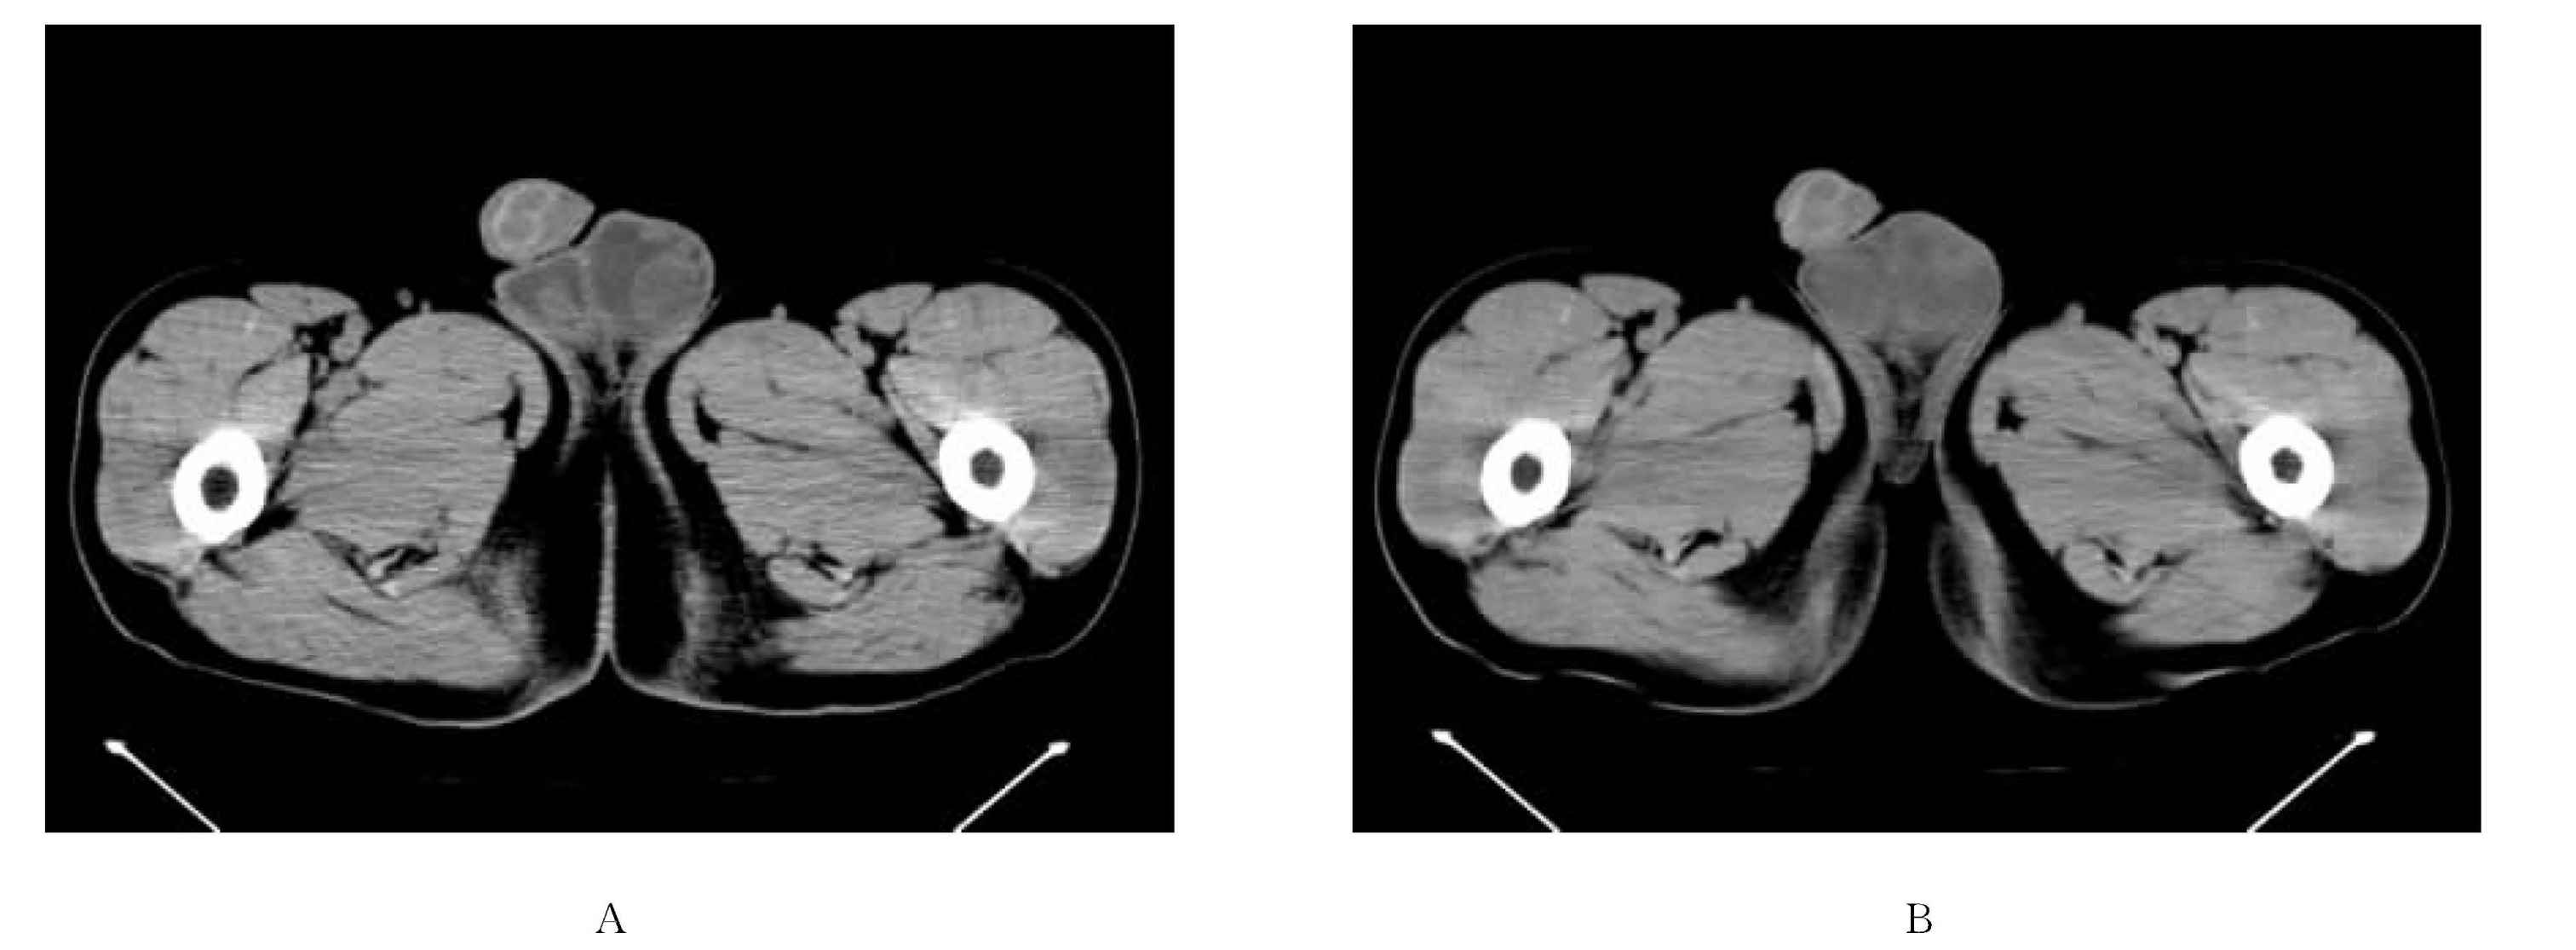
\includegraphics[width=.7\textwidth,height=\textheight,keepaspectratio]{./images/Image00404.jpg}
 \captionsetup{justification=centering}
 \caption{睾丸损伤\\{\small A、B非同一患者,A为双侧外伤性鞘膜腔积液,B为左侧睾丸内出血灶}}
 \label{fig21-8}
  \end{figure} 

上述征象的病理基础:阴囊增大主要是阴囊闭合性损伤后,鞘膜受损伤刺激黏膜分泌过多液体引起鞘膜腔积液以及睾丸损伤后水肿出血造成。其次,因阴囊间质结缔组织疏松,渗液、渗血可弥散到间质。国外有学者认为80%的阴囊血肿是睾丸破裂所致。但外伤性鞘膜腔积液多数由于睾丸破裂血液渗入所致,密度不均,CT值常在30Hu左右。肉膜损伤后水肿增厚常超过1mm,且边界模糊不清。

\section{子宫病变}

\subsection{子宫平滑肌瘤}

本病简称子宫肌瘤,是女性生殖器官中最常见的肿瘤。

\textbf{【病理】}
肿瘤可单发或多发,由平滑肌和结缔组织所组成,其外有一层疏松结缔组织假包膜。肿瘤90%起源于子宫体,5%发生在宫颈,少数位于阔韧带。按深度亦可分为黏膜下、肌层内和浆膜下,约5%~10%起源于黏膜下而突向宫腔。肿瘤大小不一,从米粒至足月妊娠大小。较大的肿瘤可因血供障碍而发生各种继发变性,如玻璃样变、囊性变、黏液样变、红色变性、坏死、钙化及脂肪变性等,有文献报道最常见的变性为玻璃样变(>60%),仅有4%发生囊性变,黏液样变则更少见。个别可恶变为平滑肌肉瘤(约0.5%)。子宫平滑肌瘤绝经后可渐萎缩,本病可合并多种良恶性病变。

\textbf{【临床表现】}
多发生于30~50岁,尤多见于不孕妇女。月经过多、月经持续时间长、间隔时间短或不规则阴道流血为主要症状。大者可有邻近脏器受压的症状。

\textbf{【CT表现】}

1.典型表现:①子宫大小及轮廓的改变:子宫外形呈分叶状增大或自子宫向外突出的实质性肿块,境界清楚,宫旁脂肪层存在(图\ref{fig21-9}A、B)。②密度:肌瘤一般密度均匀,多呈等密度,少数呈低密度,高密度少见。③肿瘤的轮廓及边缘:肿瘤大多呈圆形,边缘光滑,大的肿瘤边缘可见低密度的薄环围绕。④增强扫描:肿瘤可有不同程度的强化,多略低于正常子宫肌层的强化。

2.不典型表现:主要由于肿瘤位置特殊(子宫颈、阔韧带)、巨大及变性所致。①如发生坏死变性可见不规则的低密度区,甚至在增大增厚的肌层内呈囊性低密度区,亦可呈盆腔内巨大囊性或囊实性占位。②10%可伴斑点、条索或不规则钙化,子宫分叶状增大伴钙化对诊断有一定特异性(图\ref{fig21-9}C)。③带蒂肌瘤某些切面可显示肿块与子宫分离。④如原肌瘤突然增大或绝经后子宫扩大提示恶性变可能,但需排除妊娠或服用避孕药。⑤小的子宫肌瘤CT难以发现。

此外,还有良性转移性平滑肌瘤的报道,即组织学良性的子宫肌瘤,可出现肺内多发转移结节或腹膜后肿块(平滑肌瘤),界限清晰、密度均匀,无肿大淋巴结和腹水,强化程度不一,但良性转移性平滑肌瘤罕见。

\begin{figure}[!htbp]
 \centering
 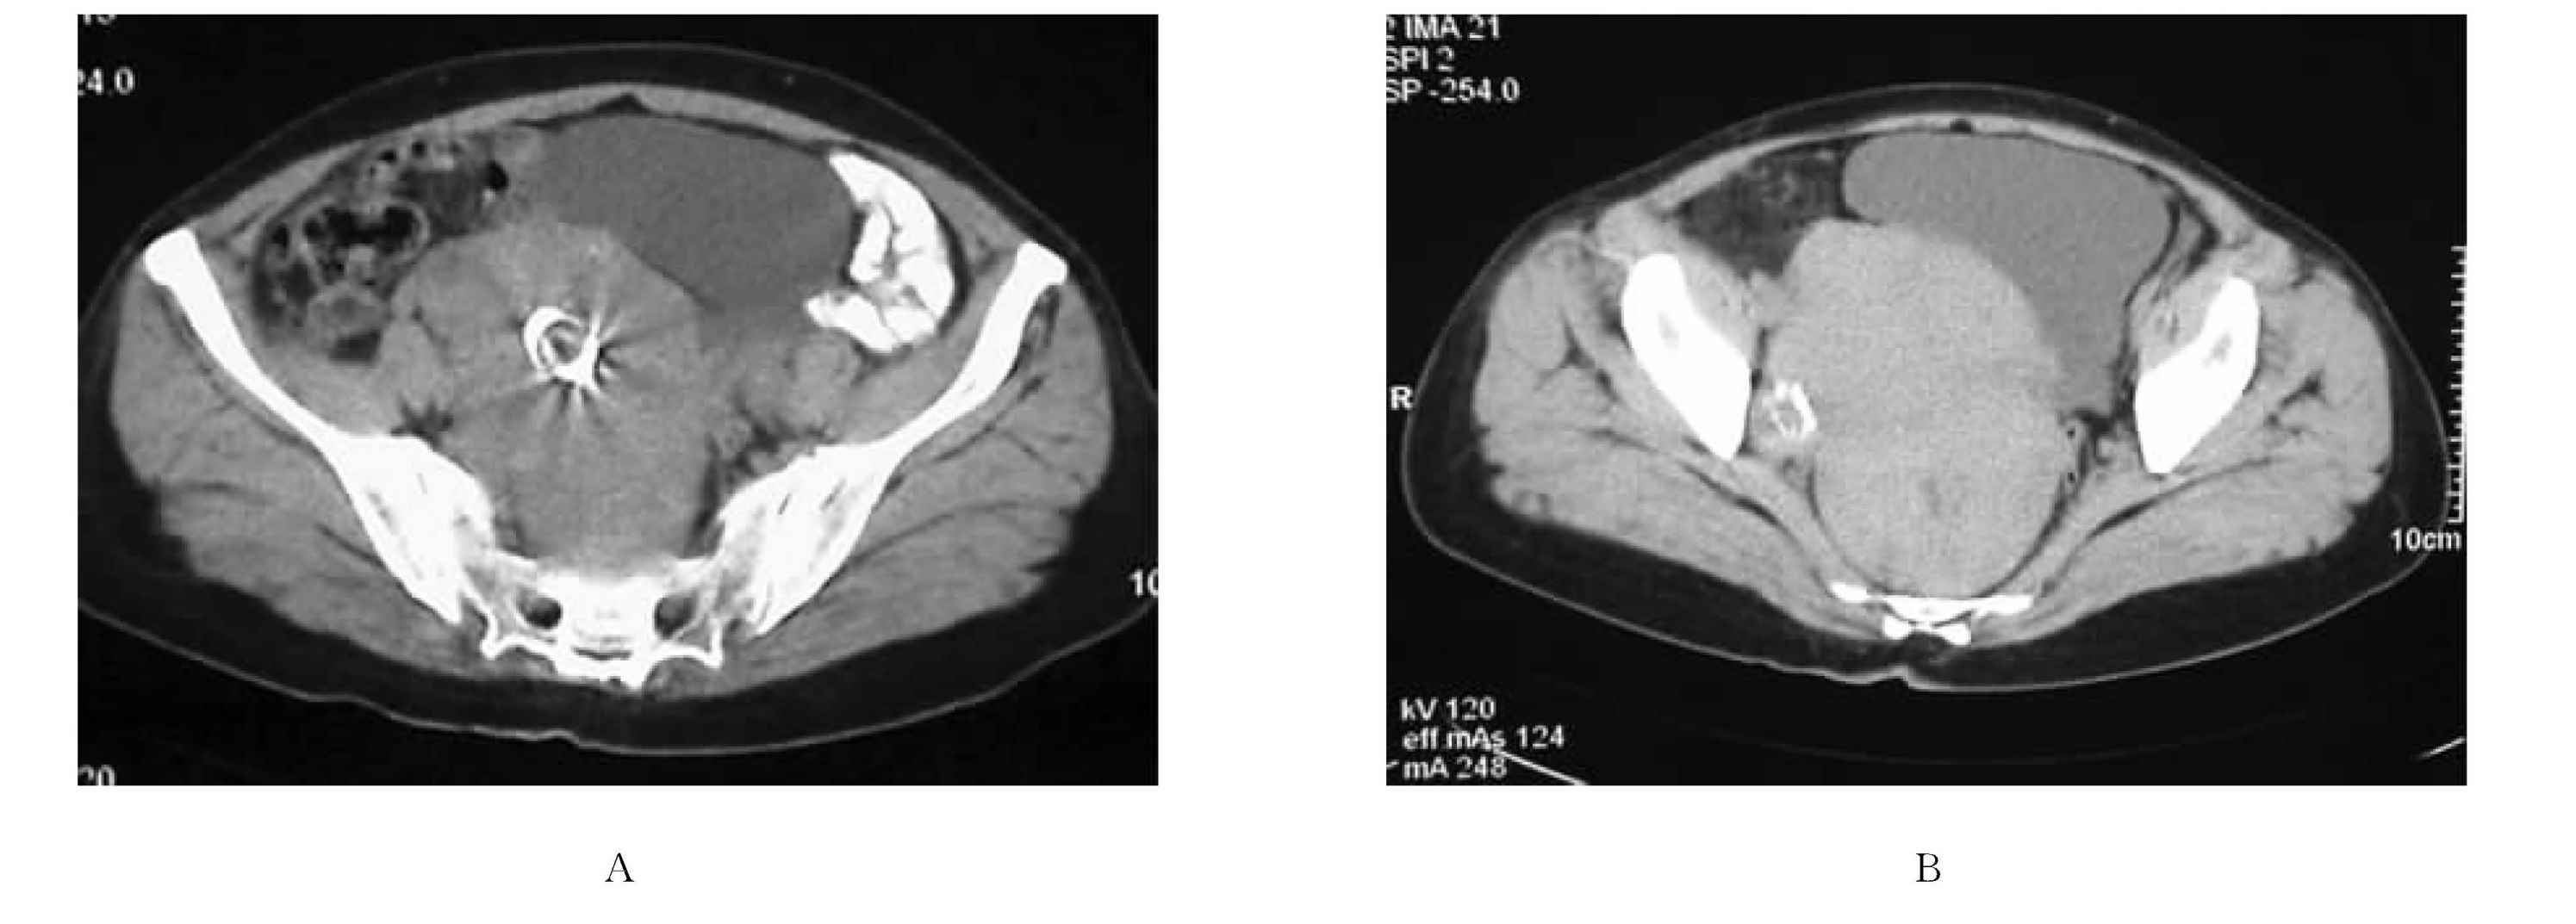
\includegraphics[width=.7\textwidth,height=\textheight,keepaspectratio]{./images/Image00405.jpg}
 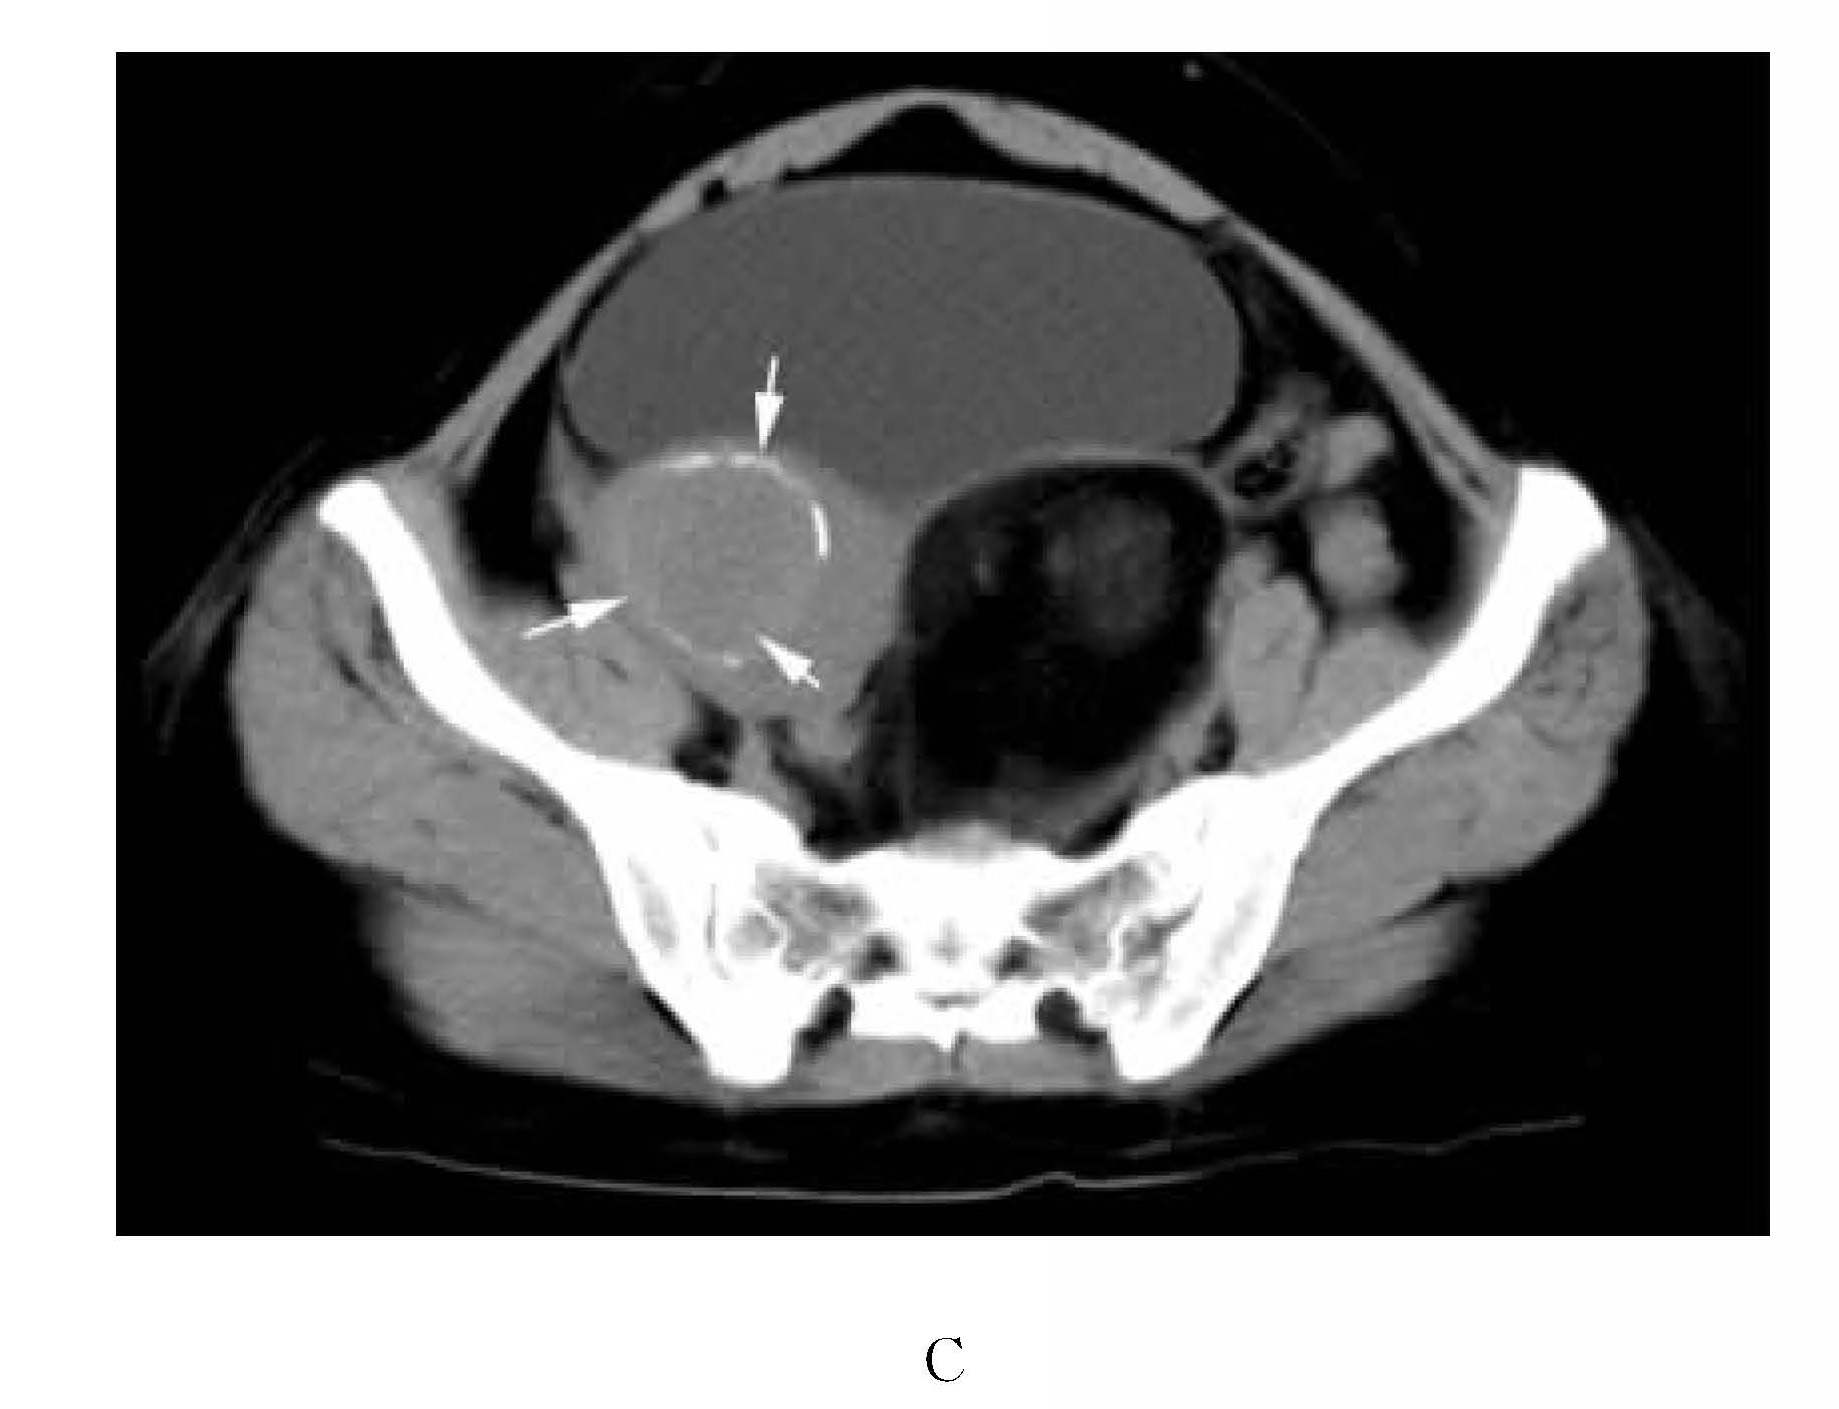
\includegraphics[width=.7\textwidth,height=\textheight,keepaspectratio]{./images/Image00406.jpg}
 \captionsetup{justification=centering}
 \caption{子宫肌瘤\\{\small A、B为同一患者,子宫后方有向外突出的等密度肿块。C示子宫内有近圆形等密度肿块,边缘钙化,子宫左侧低密度团块为卵巢畸胎瘤}}
 \label{fig21-9}
  \end{figure} 

\textbf{【鉴别诊断】}

1.子宫腺肌病:子宫腺肌病与子宫肌瘤都表现为子宫增大,病灶呈低或等密度。但前者边界不清,后者边界清楚;增强扫描子宫腺肌病尤其局限型呈点状或斑片状强化,后者未变性或钙化时呈均匀强化。

2.子宫其他肿瘤:子宫呈分叶状增大,肌层局限性增厚,宫腔变形,点状或不规则钙化,增强扫描与肌层强化一致等有助于诊断子宫肌瘤。①一些子宫肌瘤如继发变性、感染、出血、梗死可类似原发的宫颈、宫体癌,甚至难以鉴别。②伴有黏液样变的肿瘤有时难以与神经源性肿瘤鉴别,但一般后者相对较小。③浆膜下子宫肌瘤有时与卵巢肿瘤不易鉴别。④青少年女性,当CT检查发现盆腔内膀胱后上方有囊性肿块时,如果囊壁较厚,同时伴阴道扩张,又找不到正常子宫;结合患者周期性腹痛、没有初潮,可考虑诊断为处女膜阴道闭锁所致子宫阴道积血,勿误为囊变的子宫肌瘤。

此外,前屈和后屈子宫其前后径相应增大,故CT判断子宫增大应慎重。

\subsection{子宫腺肌病}

发生于正常子宫内膜部位以外的其他任何部位的子宫内膜组织称为子宫内膜异位症,多由于反复分娩损伤、流产等所致。可异位至盆腔内如卵巢(形成巧克力囊肿)、骶子宫韧带、盆腔腹膜反折、阴道直肠隔等处,亦可异位于肾、泌尿道、消化道、胸腔、体表等处,分别称为盆腔内在或外在性子宫内膜异位症。

\textbf{【病理】}
子宫内膜异位于子宫体肌层时称为子宫腺肌病。子宫腺肌病又分为两类。①弥漫型(子宫腺肌症):多见,子宫弥漫性增大,肌壁增厚。肌层内肌束增生,但无包膜,也不形成结节,其间散在由针尖至数毫米的小腔,其内充满暗红色或蓝色液体。②局限型(子宫腺肌瘤):在肌层内有单个或多个结节,无包膜,该处肌层增生夹杂出血小腔。

\textbf{【临床表现】}
好发于生育期妇女,以30~40岁多见,以继发性及逐月进行性加重的痛经为特点,患者月经紊乱。不孕是由于盆腔广泛粘连及卵巢功能异常所致,可出现性交痛和肛门坠感。

\textbf{【CT表现】}
子宫腺肌病尤其弥漫型者只能显示子宫增大,诊断意义不大。局限型者病灶呈低密度或等密度,界限不清,呈点状或斑片状强化。

有文献报道本病有21%~44%与子宫肌瘤并发,而且两者临床症状和体征相似,应注意鉴别。

\subsection{子宫颈癌}

本病是女性生殖器官中最常见的恶性肿瘤。

\textbf{【病因病理】}
本病可能与早育、多产、宫颈裂伤、宫颈糜烂及病毒作用有一定的关系。病理绝大部分为鳞状细胞癌,约占90%~95%;其次为腺癌,约占10%左右;还有其他少见类型。大体病理分为内生型、外生型和溃疡型。其主要播散途径为局部浸润、淋巴转移及血行转移。

\textbf{【临床分期】}
Ⅰ期:癌灶限于子宫颈(Ⅰa临床前期;Ⅰb临床期癌)。Ⅱ期:癌灶侵犯宫颈以外,但未累及盆壁;累及阴道上1/3段(Ⅱa无明显宫旁浸润;Ⅱb明显宫旁浸润)。Ⅲ期:病灶扩展至盆壁,已累及阴道下1/3段(Ⅲa未侵犯盆壁;Ⅲb侵犯盆壁)。Ⅳ期:肿瘤侵犯超出真骨盆或侵犯直肠、膀胱。

\textbf{【临床表现】}
以35~55岁多见,平均50岁左右,20岁以前极少发病,60岁以后发病率也有下降。早期症状可为自发或性交后阴道出血。晚期则出现阴道不规则出血、白带增多和疼痛;邻近组织器官受侵则出现相应症状和体征。

\textbf{【CT表现】}

1.肿瘤局限于子宫颈:①子宫颈增大,直径>3.5cm,边缘光整,轮廓对称或不对称(图\ref{fig21-10}A)。增强扫描呈低密度,其中可有更低密度区提示为瘤内的坏死或溃疡。②子宫颈旁未见明显的异常浸润。③输尿管末端周围脂肪间隙清晰。④子宫颈管阻塞可引起子宫腔积液。

2.宫颈旁肿瘤浸润:①子宫颈外缘不规则或模糊。②宫颈旁软组织内明显的不规则增粗条索影或软组织肿物。③输尿管末端周围脂肪间隙不清晰。但CT容易将正常的韧带、血管或子宫颈旁炎症性浸润误为宫颈旁浸润,误诊率可达40%~60%。

3.盆壁、直肠或膀胱受侵:①盆壁受侵表现为肿瘤与肌肉之间有粗条索状影相连,进而肿瘤与盆壁肌肉融合。②直肠或膀胱受侵表现为其周围脂肪层消失伴不对称性壁的增厚,进而直肠或膀胱壁有结节状或锯齿状压迹甚至腔内肿块,可有膀胱阴道瘘形成。

4.淋巴结转移:可累及宫旁淋巴结,髂内、髂外和闭孔组淋巴结,向后可累及骶前淋巴结,继而转移到髂总或主动脉旁淋巴结,甚至纵隔淋巴结。

\textbf{【术后复发的CT表现】}

术后复发可分为3型:①中央型:复发灶位于残端阴道处;②盆壁型:复发灶位于盆壁肌肉结缔组织内;③远处型。

CT表现:无论中央型还是盆壁型平扫表现为软组织肿块,缺乏特异性。增强扫描呈边缘性强化,其强化的内缘模糊,且呈边缘凹凸不平的不规则改变。有学者发现复发灶越小,强化越均匀。盆壁型需注意与盆腔内其他肿瘤相鉴别,但其他肿瘤一般无边缘性浸润性强化的特征性表现。

\textbf{【放疗后CT表现】}

①双侧宫旁呈特征性“胡须”样改变和宫旁模糊影,无盆腔侧壁改变(图\ref{fig21-10}B);②直肠旁、骶骨前间隙筋膜增厚和膀胱、直肠壁增厚;③盆腔脂肪密度增高及盆腔入口处小肠壁的增厚。

\begin{figure}[!htbp]
 \centering
 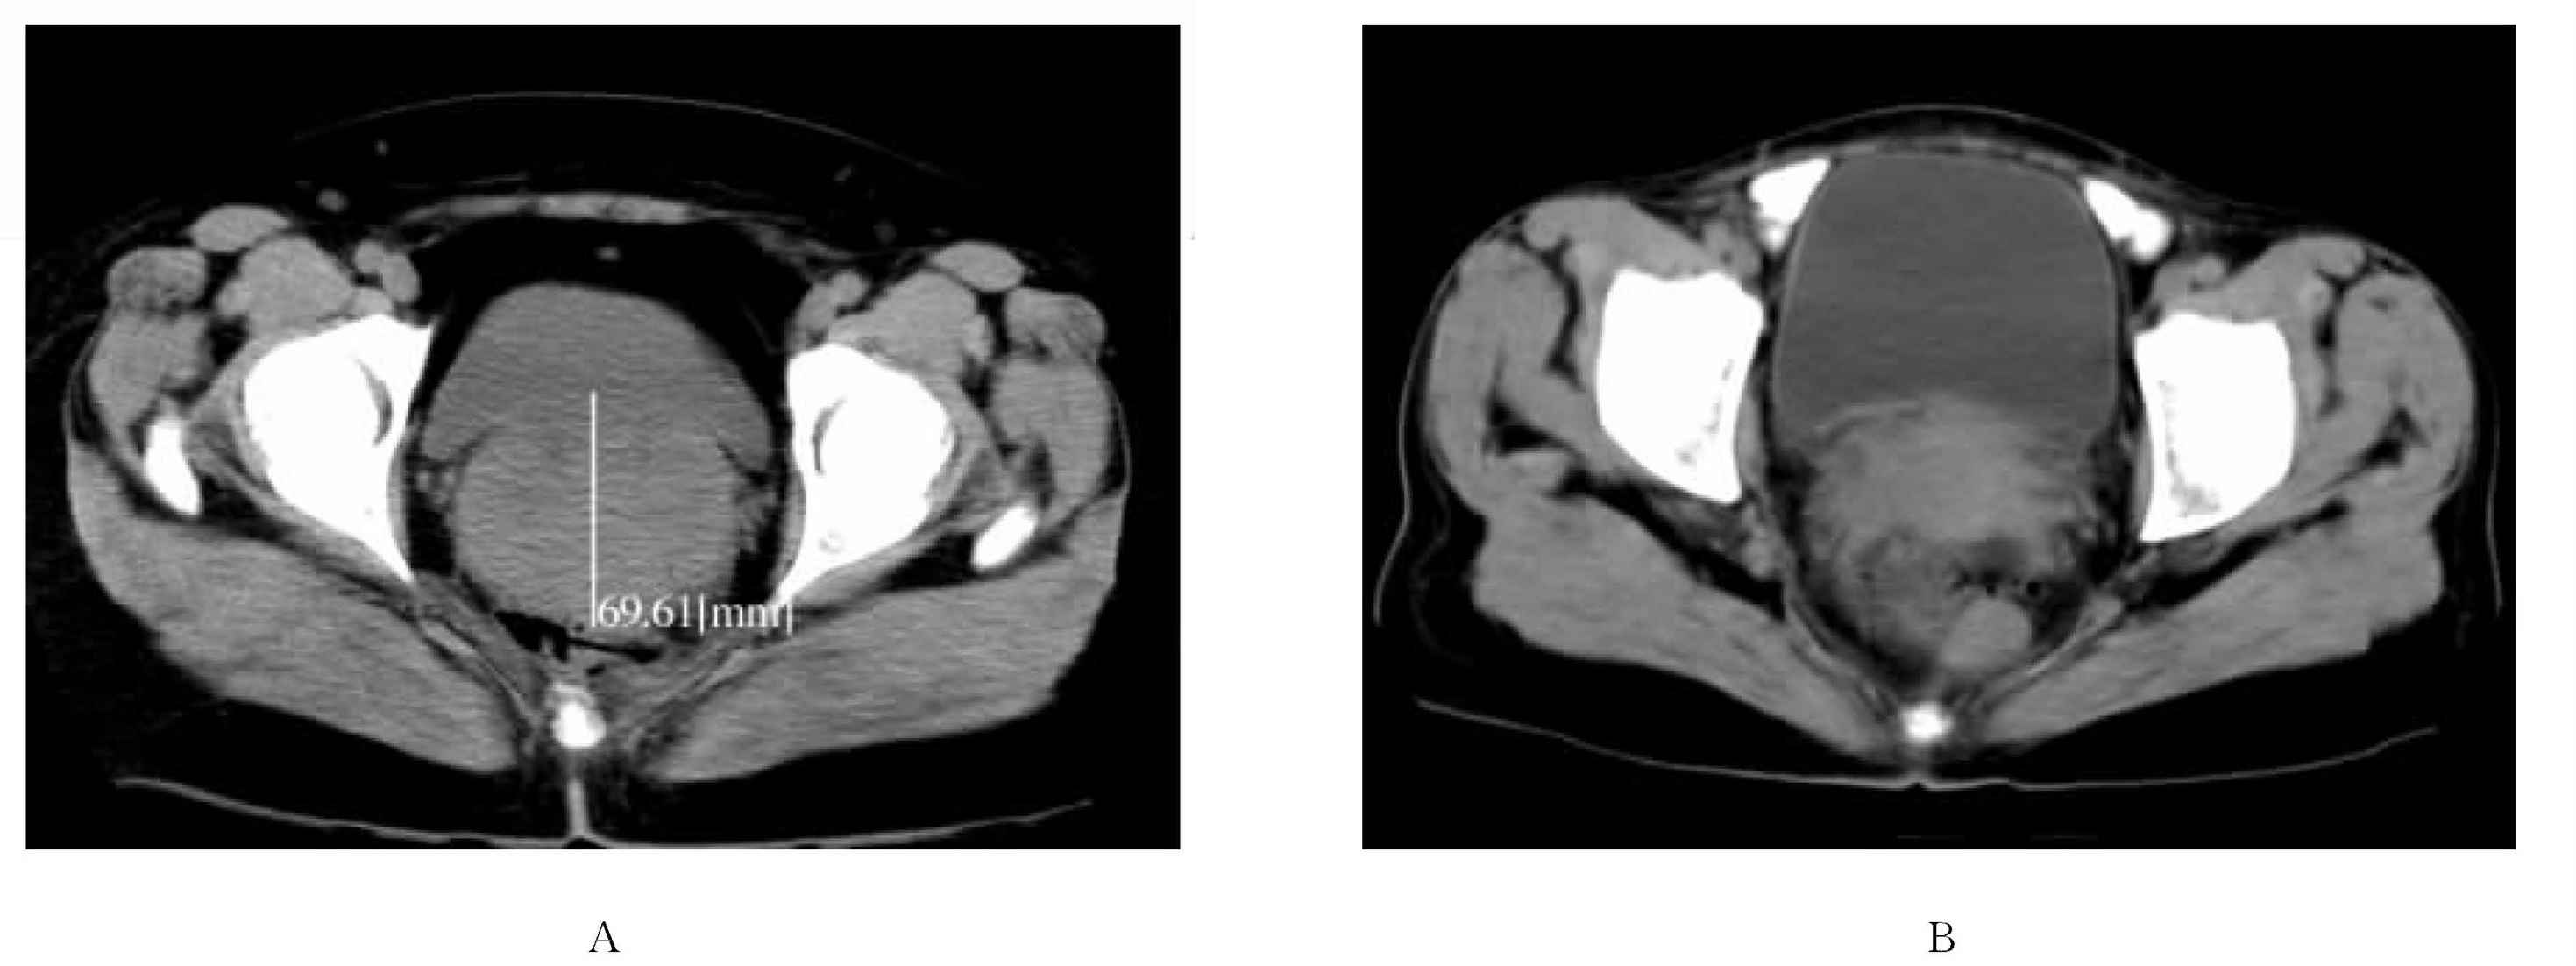
\includegraphics[width=.7\textwidth,height=\textheight,keepaspectratio]{./images/Image00407.jpg}
 \captionsetup{justification=centering}
 \caption{子宫颈癌\\{\small A、B非同一患者。A示宫颈显著增粗,界限清晰;B为宫颈癌放疗后,双侧宫旁呈“胡须”样改变和宫旁模糊影}}
 \label{fig21-10}
  \end{figure} 

但对纤维化改变与肿瘤复发的鉴别CT有一定限度,纤维化多位于宫旁,而复发一般常有盆腔和腹膜后多处肿块。

\subsection{子宫内膜癌}

本病又称子宫体癌,是指原发于子宫内膜的上皮性恶性肿瘤,其恶性程度低,发展缓慢。大多发生于50岁以上的更年期或绝经后。

\textbf{【病因病理】}
本病大部分由内分泌紊乱所致,雌激素是重要因素。其发病危险因素有肥胖、未孕、绝经晚、糖尿病、高血压、多囊卵巢综合征、卵巢肿瘤(主要是产生雌激素的颗粒细胞瘤和卵泡膜瘤)以及外源性雌激素等。

病理组织学以腺癌最多,约占75%~80%,预后较好。其他少见的有浆液性腺癌、黏液性腺癌、透明细胞癌、鳞癌、未分化癌等。大体病理分为局限型和弥漫型,以弥漫型为多。其转移途径亦分为直接蔓延、淋巴转移和血行转移。总之,本病最大特点是生长缓慢且发生转移迟缓。

\textbf{【临床分期】}
Ⅰ期:癌灶局限于子宫体;Ⅱ期:癌灶侵犯子宫体和宫颈;Ⅲ期:癌灶扩散到子宫以外,但未超出真骨盆腔范围;Ⅳ期:癌灶扩散到真骨盆腔以外或已侵犯膀胱或直肠。

\textbf{【临床表现】}
发病年龄平均55岁左右,40岁以下者仅占5%~10%。最常见的症状为阴道不规则出血,继发感染及晚期肿瘤压迫神经可出现疼痛等症状。早期可行刮宫和细胞学检查。

\textbf{【CT表现】}

1.Ⅰa期:子宫内膜癌肿位于子宫内膜内。CT表现可正常,或子宫内膜增厚,呈低密度,边缘可不规则。如果肿瘤位于一侧,则两侧的低密度内膜不对称。增强扫描肿瘤强化明显,但仍低于子宫肌层,肿瘤轮廓更清楚。

2.Ⅰb期和Ⅰc期:除Ⅰa期的表现外,子宫亦增大,肌层局部厚薄不均。增强扫描显示肿瘤边缘对肌层侵犯的深度。

3.Ⅱ、Ⅲ、Ⅳ期:①子宫腔扩大,内有软组织密度肿物,其密度低于强化的正常子宫肌。肿瘤不规则,周围可有更低密度的子宫内积液所环绕,也可充填全部子宫腔。②肿瘤侵犯肌层时正常强化的子宫肌内有局限性或弥漫性低密度,肌层变薄。③肿瘤侵犯子宫颈时,表现为子宫颈增粗、不对称、密度减低。④子宫下段、宫颈或阴道阻塞可有子宫颈积液、扩大表现。⑤肿瘤转移到附件和子宫周围时,表现为附件区及子宫颈周围囊状的低密度肿块。⑥淋巴结转移时可见髂血管周围的淋巴结增大、融合,还可见腹腔内播散表现。

\textbf{【鉴别诊断】}
子宫体低密度是一种非特异性CT表现,还可见于平滑肌瘤变性或坏死、宫腔内积液或宫颈癌侵犯到子宫内膜及其他子宫转移癌,鉴别诊断有一定限度。

\subsection{子宫肉瘤}

子宫非上皮性恶性肿瘤很少见。

\textbf{【病理】}

1.子宫平滑肌肉瘤:最多见,肉眼形态与子宫肌瘤相似,有清楚的假包膜,也可弥漫生长。

2.子宫内膜间质肉瘤:肉眼形态与腺肌病相似。

3.恶性苗勒管混合瘤:为来自多能性间质细胞的恶性混合苗勒管肿瘤,属癌肉瘤,呈息肉状突入宫腔。

\textbf{【CT表现】}
上述肉瘤的影像学表现均无特异性,可见子宫增大,病变侵及宫旁可有相应CT表现。

\subsection{子宫恶性淋巴瘤}

原发于生殖系统的恶性淋巴瘤罕见,约占结外淋巴瘤的1%。

\textbf{【病理】}
几乎均为NHL。肿瘤弥漫性侵及子宫肌层,可同时侵犯全子宫、子宫颈、阴道。整个子宫明显增大,甚至可达足月妊娠大小。

\textbf{【临床表现】}
当年轻女性,有阴道不规则流血和盆腔肿块,妇科检查有子宫颈和阴道肿物及溃疡时应考虑到淋巴瘤的可能。

\textbf{【影像学表现】}
无特异性,可见子宫体、宫颈或阴道呈等密度弥漫性增大,且仍大致保持“正常”形态结构,密度多均匀。

\subsection{葡萄胎}

本病又称水泡状胎块、良性葡萄胎。其病因及本质尚不明确,一种观点认为是肿瘤性疾病,另一种观点认为是胎儿发育障碍死亡后所致。

\textbf{【病理】}
以胎盘绒毛间质高度水肿,滋养层细胞不同程度增生为特征。大体病理见全部或部分绒毛呈半透明水泡状、大小不等,其间有细蒂相连成串,状如葡萄故称葡萄胎。主要发生于宫腔及蜕膜层。良性葡萄胎可转换为侵袭性葡萄胎(即侵入子宫肌层深部或转移至近处或远处器官),其相隔的时间不一,但多在葡萄胎清除后6个月内发生。

\textbf{【临床表现】}
①闭经:绝大多数有此症状,闭经时间多为8~12周或更长;②阴道流血:为不规则流血,如在流出的血液中发现水泡状物,诊断即明确;③腹痛:可有阵发性腹痛,为子宫阵发性收缩所致;④子宫增大异常:多比正常妊娠月份大,但也有不大甚至小者;⑤黄素囊肿;⑥妊娠高血压综合征;⑦贫血与感染。

\textbf{【CT表现】}
子宫体积较同孕期妊娠月份大,宫腔扩大,腔内呈不均质的混杂密度灶。增强扫描子宫壁明显强化,宫腔内胎盘绒毛间质因少血管而呈轻度强化。可表现为宫腔内水泡状或雪花状特征性改变,这是间质和小泡相互衬托下所致。水泡状表示水泡较大,绒毛间质相对较少;反之,水泡较小,绒毛间质相对较多则呈雪花状。胎盘与宫壁分界清晰,增强扫描胎盘与宫壁间有时可看到水样分界线,则有利于与侵袭性(恶性)葡萄胎鉴别。此外,约25%~60%可合并卵巢黄素囊肿。

\textbf{【鉴别诊断】}
一般孕龄8周前,子宫体积增大,宫壁增厚,密度均匀;宫腔扩大,腔内均匀水样密度影,胚胎组织尚均匀,仅大小有别。当在8周末时,胎盘密度可不均匀,但羊膜囊密度始终为均匀一致的水样密度,其范围可随胚胎组织的增大而缩小。

\subsection{侵袭性葡萄胎}

本病又称为恶性葡萄胎或破坏性绒毛膜腺瘤。大多继发于葡萄胎之后,也可开始即为侵袭性,或者说葡萄胎组织侵入子宫肌层深部或转移至近处或远处器官,即为侵袭性葡萄胎。

\textbf{【病理】}
葡萄胎组织侵入子宫肌层深部。胎盘绒毛水肿、液化、增生,变成无数大小不等的透明水泡样物,充满子宫腔。病灶穿破肌壁处可引起出血灶,其中含有一定异型性滋养细胞的水泡状绒毛。

\textbf{【临床表现】}
①阴道流血或内出血:葡萄胎清除后,阴道持续不规则出血;子宫略大而软,经再次刮宫排除葡萄胎组织残留后,仍不见好转;如瘤组织穿破子宫浆膜层,可引起腹腔内出血,因而引起腹痛。②转移灶表现:最常见的肺转移可致咳嗽、咯血;转移至子宫颈、阴道、消化道、脑等部位可有相应的症状和体征。

\textbf{【CT表现】}
①平扫:子宫不同程度增大,腔内充填水样密度影夹杂不同分布的斑点状、片状及环形边缘模糊的等密度影,有的可见条片状出血灶。腔内壁轮廓线均有不同范围的局限性消失。②增强扫描:由于肿瘤血运丰富,腔内平扫的等密度(软组织)灶显著强化。部分呈小圆形低密度环形强化称为“葡萄征”;部分融合成不规则的一簇,形似“火焰山”,边缘模糊;还可见腔内壁轮廓线消失处肌层呈不均质强化。③远处转移:可有肺、消化道、脑等部位的转移。④可合并一侧或双侧卵巢黄素囊肿,且刮宫后逐渐增大(一般黄素囊肿刮宫后变小)。

\subsection{绒毛膜癌}

绒毛膜癌是来自绒毛膜滋养层上皮的一种高度恶性肿瘤。绝大多数与妊娠有关,约40%~60%发生于葡萄胎后,20%~30%发生于流产后,其余病例发生于早产或正常分娩后。发病年龄以30岁左右为多。

\textbf{【病因病理】}
绒癌的发生原因不清,一般认为葡萄胎、侵袭性葡萄胎及绒癌是绒毛滋养层细胞增生由良性到恶性的肿瘤过程。有文献认为,葡萄胎排出1年以上恶变者应诊断为绒毛膜癌;6个月内恶变者则应诊断为侵袭性葡萄胎;6个月至1年内恶变者则侵袭性葡萄胎和绒癌的可能各占一半。

绒癌的肿瘤多位于子宫底前后壁,突入宫腔或向肌层浸润,甚至穿透浆膜。有时瘤体位于子宫肌内,也可侵及子宫颈、阴道、输卵管或阔韧带。瘤组织中由两种异型性明显的细胞组成:一种为类似细胞滋养层细胞,另一种为融合体细胞滋养层细胞。出血、坏死非常明显。瘤组织中无血管及其他间质组织存在,也无绒毛样结构形成,这一点有别于恶性葡萄胎。

\textbf{【临床表现】}
与侵袭性葡萄胎类似,主要有阴道流血及内出血、转移症状(常见为肺和阴道转移)。盆腔检查子宫增大、有时外形不规则等。

\textbf{【CT表现】}
无特征性。子宫大小正常或增大,有不规则低密度或高密度出血区。平扫和增强扫描可见子宫壁受侵,甚至宫旁受侵,可有远处转移表现。与侵袭性葡萄胎一样,常合并单侧或双侧卵巢黄素囊肿,且在刮宫后继续增大。

总之,滋养细胞肿瘤常根据临床表现及化验检查即可做出诊断,极少需做CT、MR检查。B超对侵袭性葡萄胎诊断价值很大。

\subsection{子宫脂肪类肿瘤}

该类肿瘤包括单纯脂肪瘤、纤维平滑肌脂肪瘤及脂肪细胞肉瘤样变,十分罕见,占子宫肿瘤的0.03%~0.2%,多见于50岁以上。

\textbf{【病理】}
肿瘤的组织学起源不同,大小多为5~10cm,常有完整包膜,发病部位以子宫肌壁间较多,也可发生于子宫颈或阔韧带。

\textbf{【CT表现】}
由于肿瘤中有成熟的脂肪组织,表现为边缘清楚的含脂肪成分的肿块而得以提示诊断。但确切诊断靠病理组织学。

\subsection{子宫转移癌}

本病为妇科恶性肿瘤,尤其是卵巢癌、宫颈癌可侵犯或转移至子宫。其他非妇科肿瘤转移至子宫者可来自乳腺、胃、结肠、胰腺、肾,亦可来自黑色素瘤。

转移瘤可累及子宫内膜或肌层,常有不规则阴道出血。影像学不能与原发性子宫内膜癌相鉴别。

\section{卵巢病变}

\subsection{概述}

卵巢肿物常见,是女性盆腔肿块的重要原因,主要包括非肿瘤性的卵巢巧克力囊肿和卵巢囊肿,以及各种类型的良、恶性肿瘤。

卵巢肿瘤约80%为良性,多见于育龄妇女,以囊腺瘤或成熟的畸胎瘤(主要为皮样囊肿,也可为实性)最常见;卵巢囊腺瘤在绝经前的良性肿瘤中约占50%,绝经后约占80%。卵巢囊腺癌则为最常见的恶性肿瘤。卵巢肿瘤基本上分为生发上皮性肿瘤、性索间质肿瘤和生殖细胞肿瘤3大类。

良性肿瘤主要有:①来源于生发上皮的浆液性和黏液性囊腺瘤。②来源于生殖细胞的皮样囊肿。③来源于性索间质的有纤维瘤、卵泡膜细胞瘤。

恶性肿瘤主要有:①来源于生发上皮的有浆液性囊腺癌(42%)、黏液性囊腺癌(12%)、子宫内膜癌(15%)、未分化癌(17%)、透明细胞癌(6%)。②来源于生殖细胞的有无性细胞瘤、不成熟畸胎瘤(即恶性畸胎瘤)、内胚窦瘤(又称卵黄囊瘤)、胚胎癌、绒毛膜癌。③来源于间质的以颗粒细胞瘤多见。此外,还有淋巴瘤和转移瘤等。

\subsection{卵巢及盆腔内子宫内膜异位症}

发生于正常子宫内膜部位以外的其他任何部位的子宫内膜组织称为子宫内膜异位症。

\textbf{【病因病理】}
多由于反复分娩损伤、流产等所致。卵巢子宫内膜异位症占子宫外子宫内膜异位症的80%,常为双侧性。如病灶内出血则产生卵巢的宫内膜囊肿,由于囊内含有陈旧性积血呈巧克力样糊状物,因此这种囊种又称为卵巢巧克力囊肿。在此基础上可发生卵巢的子宫内膜恶性肿瘤。囊肿一般5~6cm大小,最大可达25cm。

但也有学者认为其他卵巢囊肿出血,其内容物亦可呈巧克力状,故卵巢巧克力囊肿并非子宫内膜异位症所特有。

\textbf{【临床表现】}
主要症状为继发性及逐月进行性加重的痛经、月经紊乱。不孕是由于盆腔广泛粘连及卵巢功能异常所致。异位至盆腔内其他部位,以及肾、泌尿道、消化道等处,可出现肠道及尿路症状。

\textbf{【CT表现】}
①多为囊性,少数呈实性或囊实性,囊性和囊实性相对表现典型。②多发病变,由反复出血所致。出血的时间不一,而致密度不一;既可为水样密度,也可为高密度囊肿(图\ref{fig21-11})。③病变轮廓不光整,边缘模糊;肿物与邻近的子宫、膀胱、输尿管、直肠边界不清,由粘连所致。④增强扫描实性部分有近中度强化。

\begin{figure}[!htbp]
 \centering
 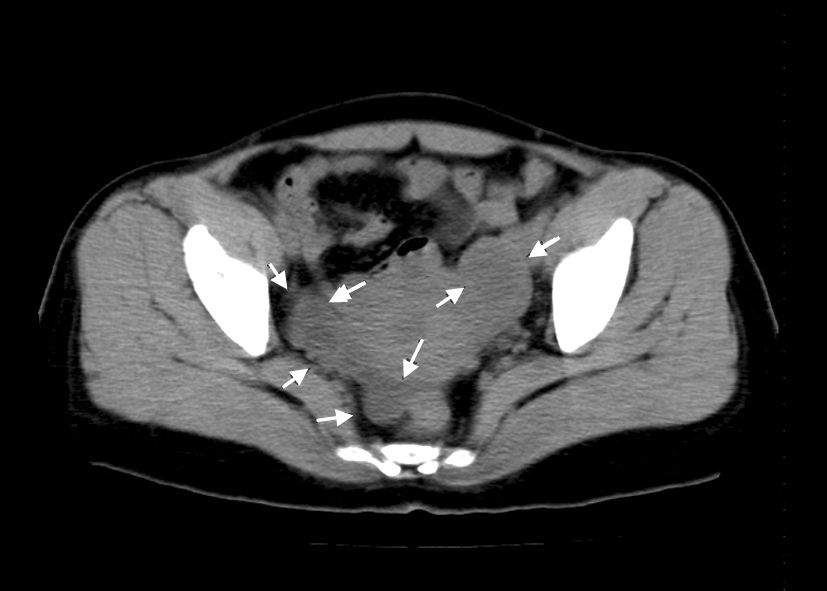
\includegraphics[width=.7\textwidth,height=\textheight,keepaspectratio]{./images/Image00408.jpg}
 \captionsetup{justification=centering}
 \caption{卵巢及盆腔内子宫内膜异位症\\{\small 左右侧附件区可见多个囊状水样低密度灶,病灶长径与同侧盆壁近乎平行}}
 \label{fig21-11}
  \end{figure} 

国内有学者报道,本病有以下特征:病灶上缘常不超过子宫上缘,且2/3的病灶长径与同侧盆壁近乎平行,50%的病灶长径大于横径达1.5倍;表现为多房样囊肿,占据子宫、直肠与盆壁之间的狭长间隙。此外,还有文献认为囊腔内片状高密度灶(为新鲜凝血块)是其特征性表现;囊壁厚而毛糙,囊液高密度或高低混杂密度,出现类液平面、分层征亦有一定特征性。实块型与肿瘤、肉芽肿鉴别困难。

\subsection{卵巢囊肿}

\textbf{【病理】}
主要为两类:①单纯囊肿;②功能性囊肿:与排卵有关,包括滤泡囊肿、黄体囊肿及黄素囊肿等。囊肿多为单个,直径一般<5cm。部分为多发或两侧同时有囊肿,也可能较大。多为单房、壁菲薄、边缘光滑,无分隔及软组织成分,囊液稀薄。

\textbf{【临床表现】}
常无症状,功能性者可有月经异常。较大者可有坠胀感或压迫症状。

\textbf{【CT表现】}
典型表现为附件或子宫直肠窝区圆形或椭圆形囊性肿块,边缘光滑、界限清晰;直径多<5cm;囊肿密度均匀,CT值近于水;壁菲薄而通常不能显示,内无间隔或软组织成分。无乳头状突起和结节状间隔对诊断和鉴别诊断甚为重要。

但大部分囊肿并不十分典型,①囊液密度较高,部分CT值高达40Hu左右,与囊内出血或部分容积效应有关;囊肿出血可呈均匀、条片状、新月形密度增高区,CT值可达30~60Hu;②囊肿与正常卵巢交界处局限性囊壁增厚,或出现细条状单个甚至多个间隔;③囊壁不规则增厚及乳头状软组织突起。不典型者与囊腺瘤或囊腺癌可不易鉴别。

\subsection{多囊卵巢综合征}

有文献将本病归为卵巢功能性囊肿。

\textbf{【病因病理】}
其病因不明,可能由于下丘脑的功能紊乱,引起肾上腺及卵巢功能失调所致。促黄体生成激素分泌增多,抑制排卵,使卵巢有很多滤泡聚集、双侧卵巢对称性增大。

\textbf{【临床表现】}
为继发性的月经稀少,继而闭经。患者闭经、多毛、肥胖,妇科检查可扪及增大的卵巢。

\textbf{【影像学表现】}
①盆腔充气造影:可显示双侧卵巢对称性增大,为正常卵巢的2~3倍,且保持原来外形。②CT与B超均无特征性,仅可显示双侧卵巢增大,难以显示小囊肿。MRT\textsubscript{2}
WI可显示其小的囊肿。

\subsection{卵巢浆液性和黏液性囊腺瘤}

\textbf{【病理】}

1.浆液性囊腺瘤:占卵巢良性肿瘤的25%,双侧发生者约10%。

肿瘤以单房为主,多房者少见。囊液稀薄,呈草黄色或棕色。囊壁内面光滑,部分伴乳头状软组织突起。肿瘤间质或乳头状组织中可有钙盐沉着,形成砂粒体是其特征。恶变率可达30%~50%。

2.黏液性囊腺瘤:占卵巢良性肿瘤的20%,双侧发生者占5%,是人体中最大的肿瘤之一。

肿瘤表面光滑,呈灰白色,约半数为多房性,内含草绿色或棕色黏液。若囊壁破裂,内容物流入腹腔,可种植于腹腔产生大量黏液,即“腹膜假性黏液瘤”。恶变率低于浆液性,为5%~10%,多见于绝经后。

\textbf{【临床表现】}
浆液性囊腺瘤多见于30~40岁;黏液性囊腺瘤多见于25~45岁。主要表现为盆腔肿块,较大肿块可产生压迫症状,造成大小便障碍等。

\textbf{【CT表现】}

1.浆液性囊腺瘤:①多为单房囊性肿块,内为均匀水样密度,少数可为多房。②囊壁薄而均匀,囊壁及间隔厚度<3mm。③肿瘤一般较大,直径可达10cm左右。④可有囊壁乳头状软组织突起及厚壁表现,但含量少,且不多见。⑤少数可见囊壁内或软组织中有沙砾样钙化。⑥囊内出血可呈均匀或条索状、新月形密度增高区。

2.黏液性囊腺瘤:①常为多房囊性肿块,囊液黏稠,CT值高于水,但低于软组织,CT值10~26Hu(图\ref{fig21-12}),囊内出血可有相应密度增高的表现。②囊壁较薄,但欠均匀,囊内常见由多个细条样间隔形成的多个小囊,囊壁及间隔亦多<3mm。③肿瘤一般较浆液性大,直径多>10cm。④软组织乳头状突起较浆液性少见。如果瘤内出现实性成分,则提示恶性可能。⑤如囊壁破裂产生大量黏液,形成腹膜假性黏液瘤而产生相应表现。

\begin{figure}[!htbp]
 \centering
 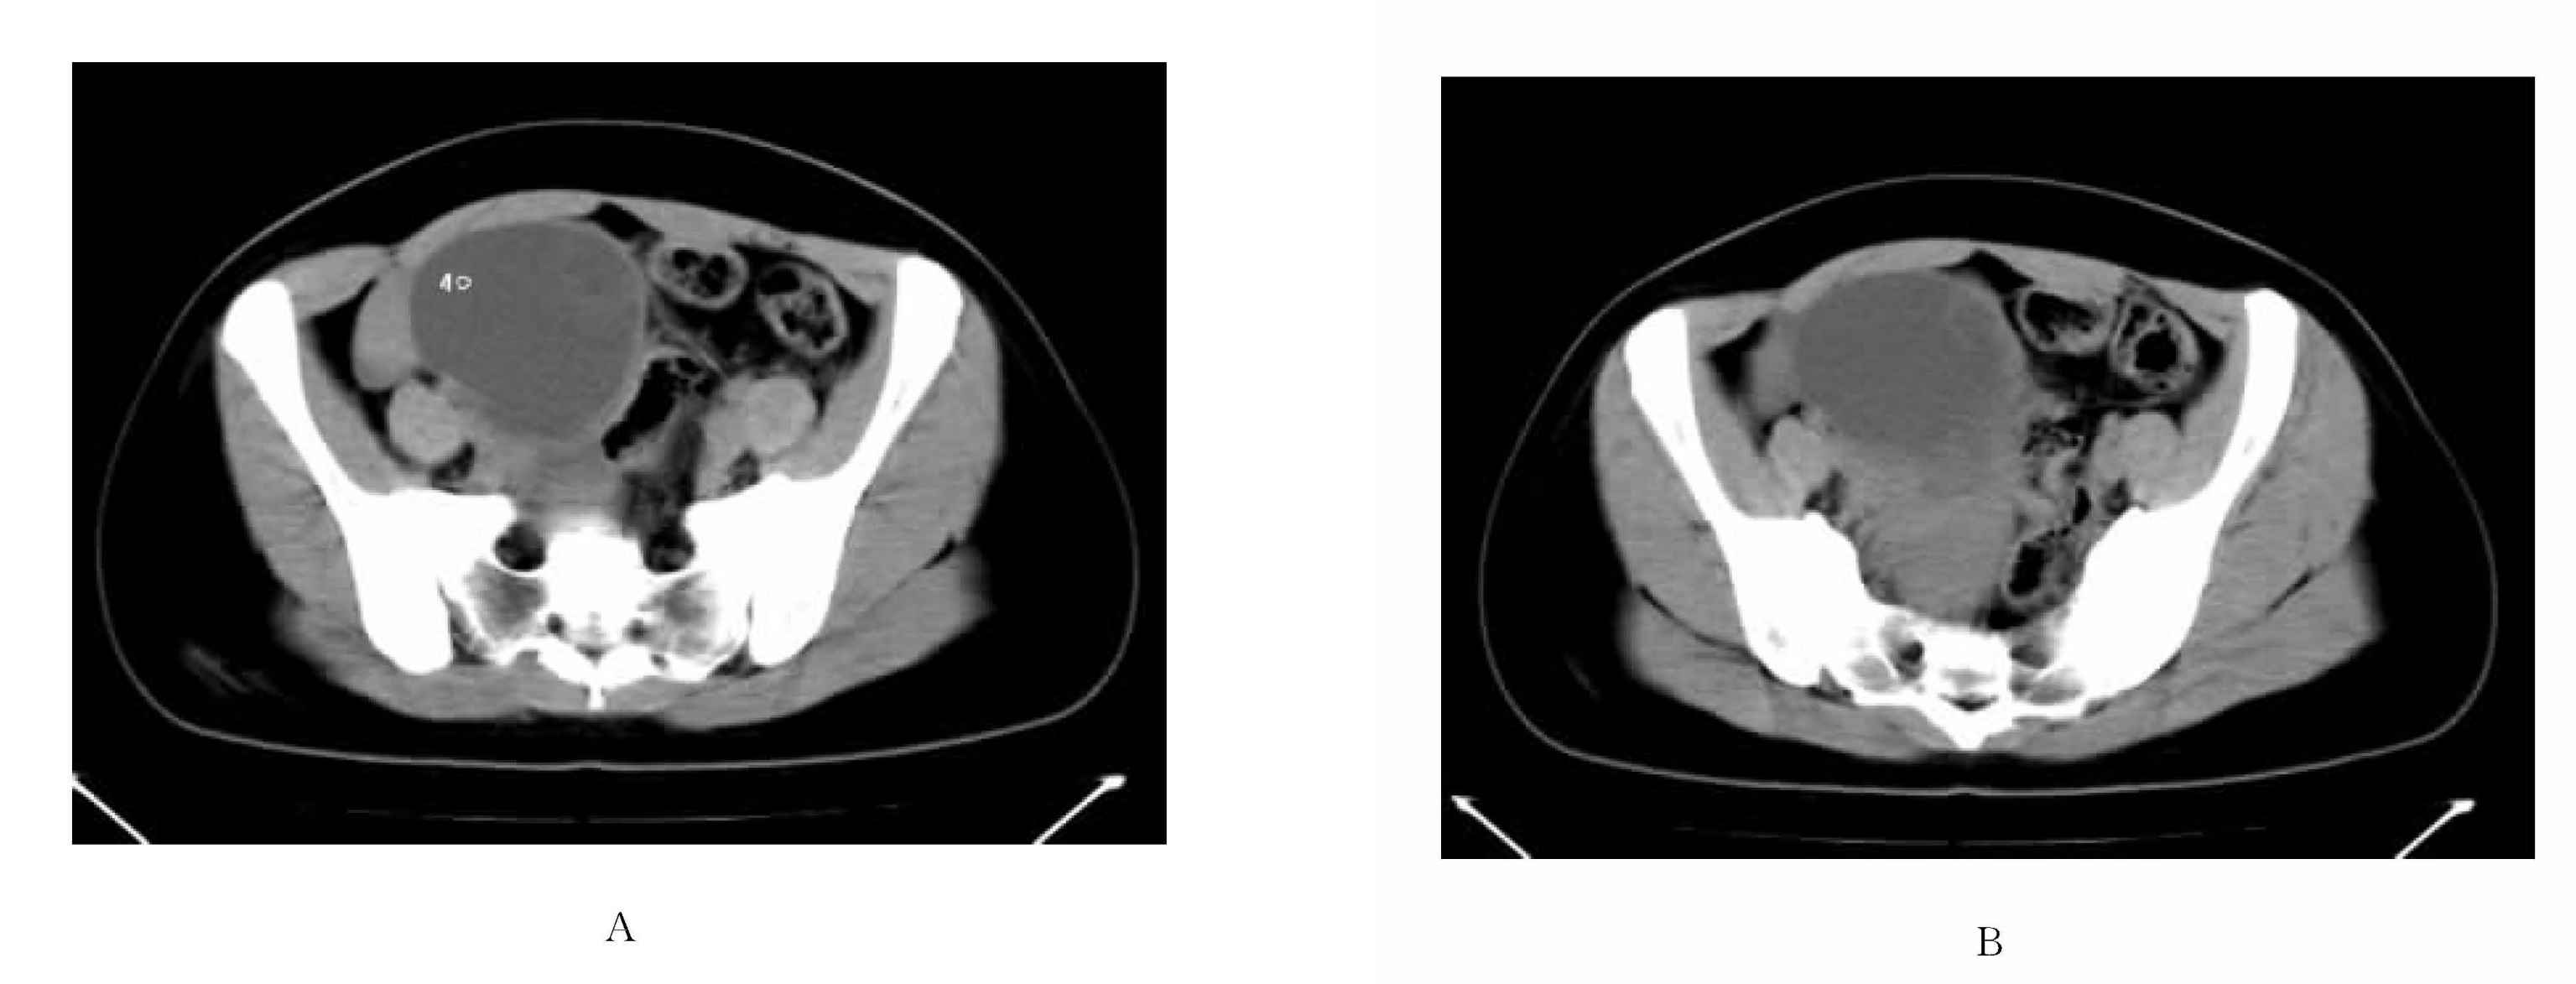
\includegraphics[width=.7\textwidth,height=\textheight,keepaspectratio]{./images/Image00409.jpg}
 \captionsetup{justification=centering}
 \caption{卵巢黏液性囊腺瘤\\{\small A、B为同一患者,盆腔内囊状水样密度灶,界限清晰,囊壁薄而规整}}
 \label{fig21-12}
  \end{figure} 

\textbf{【鉴别诊断】} 应注意与卵巢囊腺癌相鉴别(见表\ref{tab21-1})。

\begin{table}[htbp]
\centering
\caption{卵巢囊腺瘤与囊腺癌的CT鉴别诊断}
\label{tab21-1}
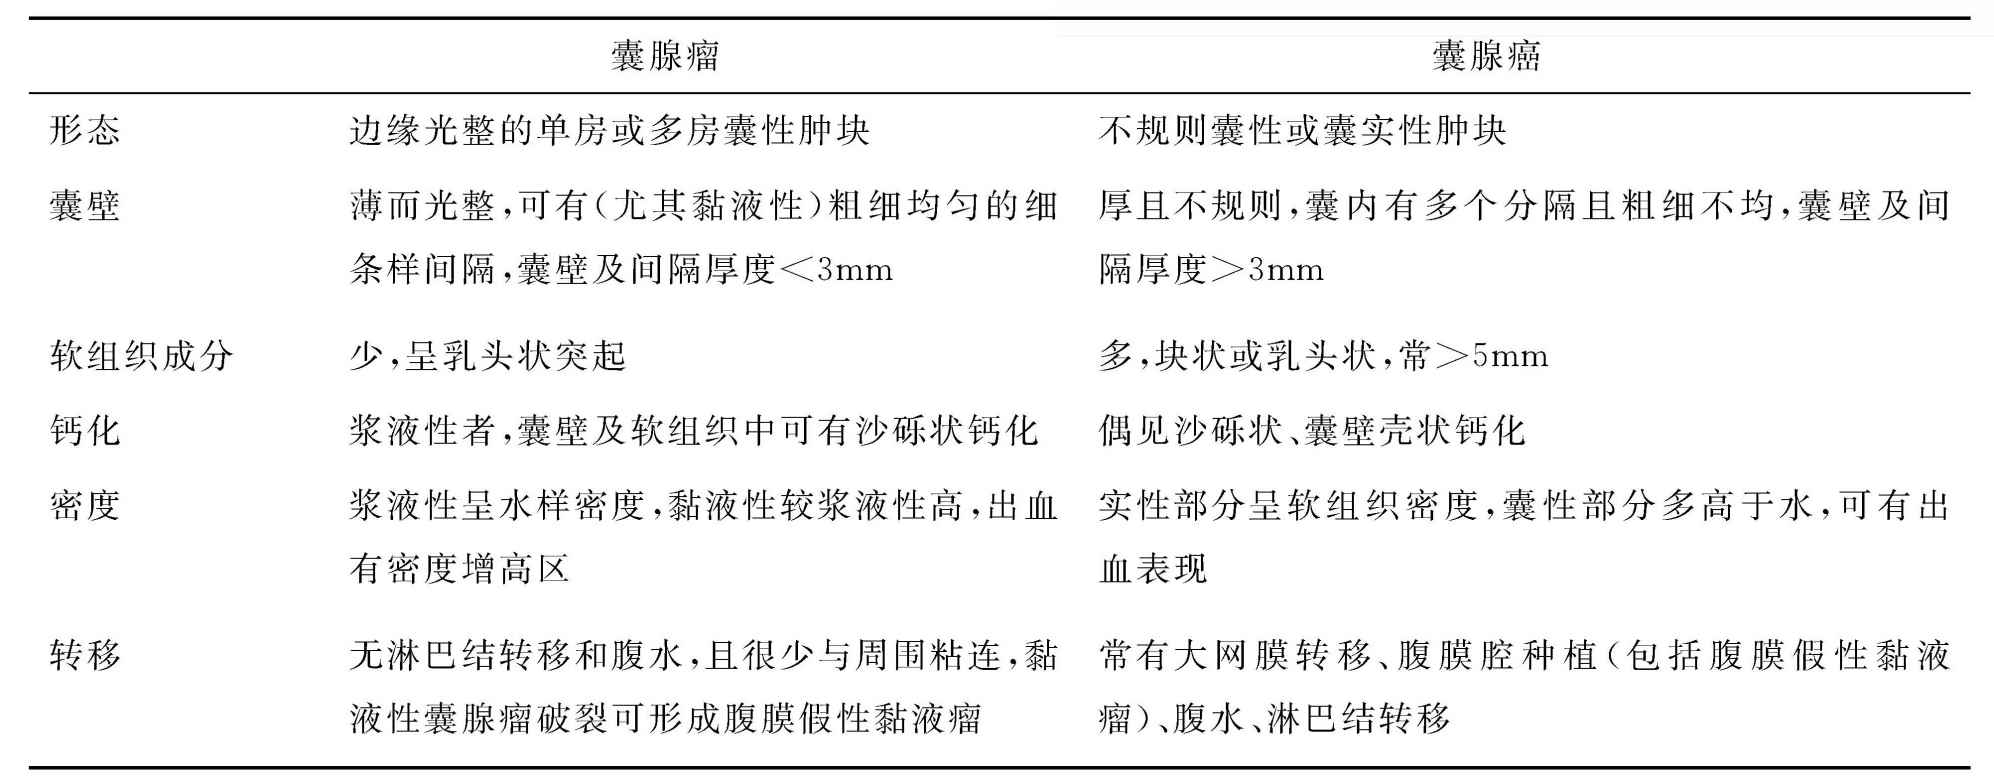
\includegraphics[width=\textwidth,height=\textheight,keepaspectratio]{./images/Image00410.jpg}
\end{table}

\subsection{卵巢畸胎瘤}

本病占所有卵巢肿瘤的11%~20%,占生殖细胞肿瘤的90%以上。其中97%为囊性成熟性,其余为未成熟性或单胚层高度特异性。

\textbf{【病理】}

1.成熟性畸胎瘤:由分化好的外、中、内胚层来源的组织构成,以外胚层成分最多。肿瘤多数为单侧性,双侧性占8%~15%。几乎均为囊性,呈圆形、卵圆形或分叶状,表面光滑,多呈单房,内含毛发和皮脂样物。镜下外壁为卵巢间质,内衬皮肤、毛发和皮肤附件。囊内壁常可见1个或多个大小不等的实性或囊实性突起,称为头结节。头结节表面有毛发及牙齿,切面可见骨、软骨和脂肪组织,镜下为3个胚层的多种组织。恶变率占2%,常为鳞癌、腺癌和类癌。

2.未成熟畸胎瘤:以实性为主,伴有囊性区,前者由来自3个胚层的成熟或未成熟组织(主要为神经上皮组织)构成。

3.单胚层高度特异性肿瘤:包括卵巢甲状腺肿、类癌、神经外胚层肿瘤和皮脂腺肿瘤等。以卵巢甲状腺肿多见,切面为被纤维分隔的甲状腺和少量胶样物。

\textbf{【临床表现】}
肿瘤多见于育龄期妇女,平均34岁,其中未成熟性发病年龄<20岁。通常无症状,大者可触及肿块,良性者发生扭转时或恶性者可疼痛。较大肿块可产生压迫症状。

\textbf{【CT表现】}

1.成熟性畸胎瘤:几乎全为囊性,大多数直径为4~15cm,少数1~2cm或巨大,93%~96%的肿瘤内可见脂肪密度为特征性表现(图\ref{fig21-13})。此外,液脂面表现也具有一定特征,当液-脂面上有漂浮物时,液面呈抛物线状。虽脂肪瘤等含有脂肪,但因非常罕见,一般不予考虑。

\begin{figure}[!htbp]
 \centering
 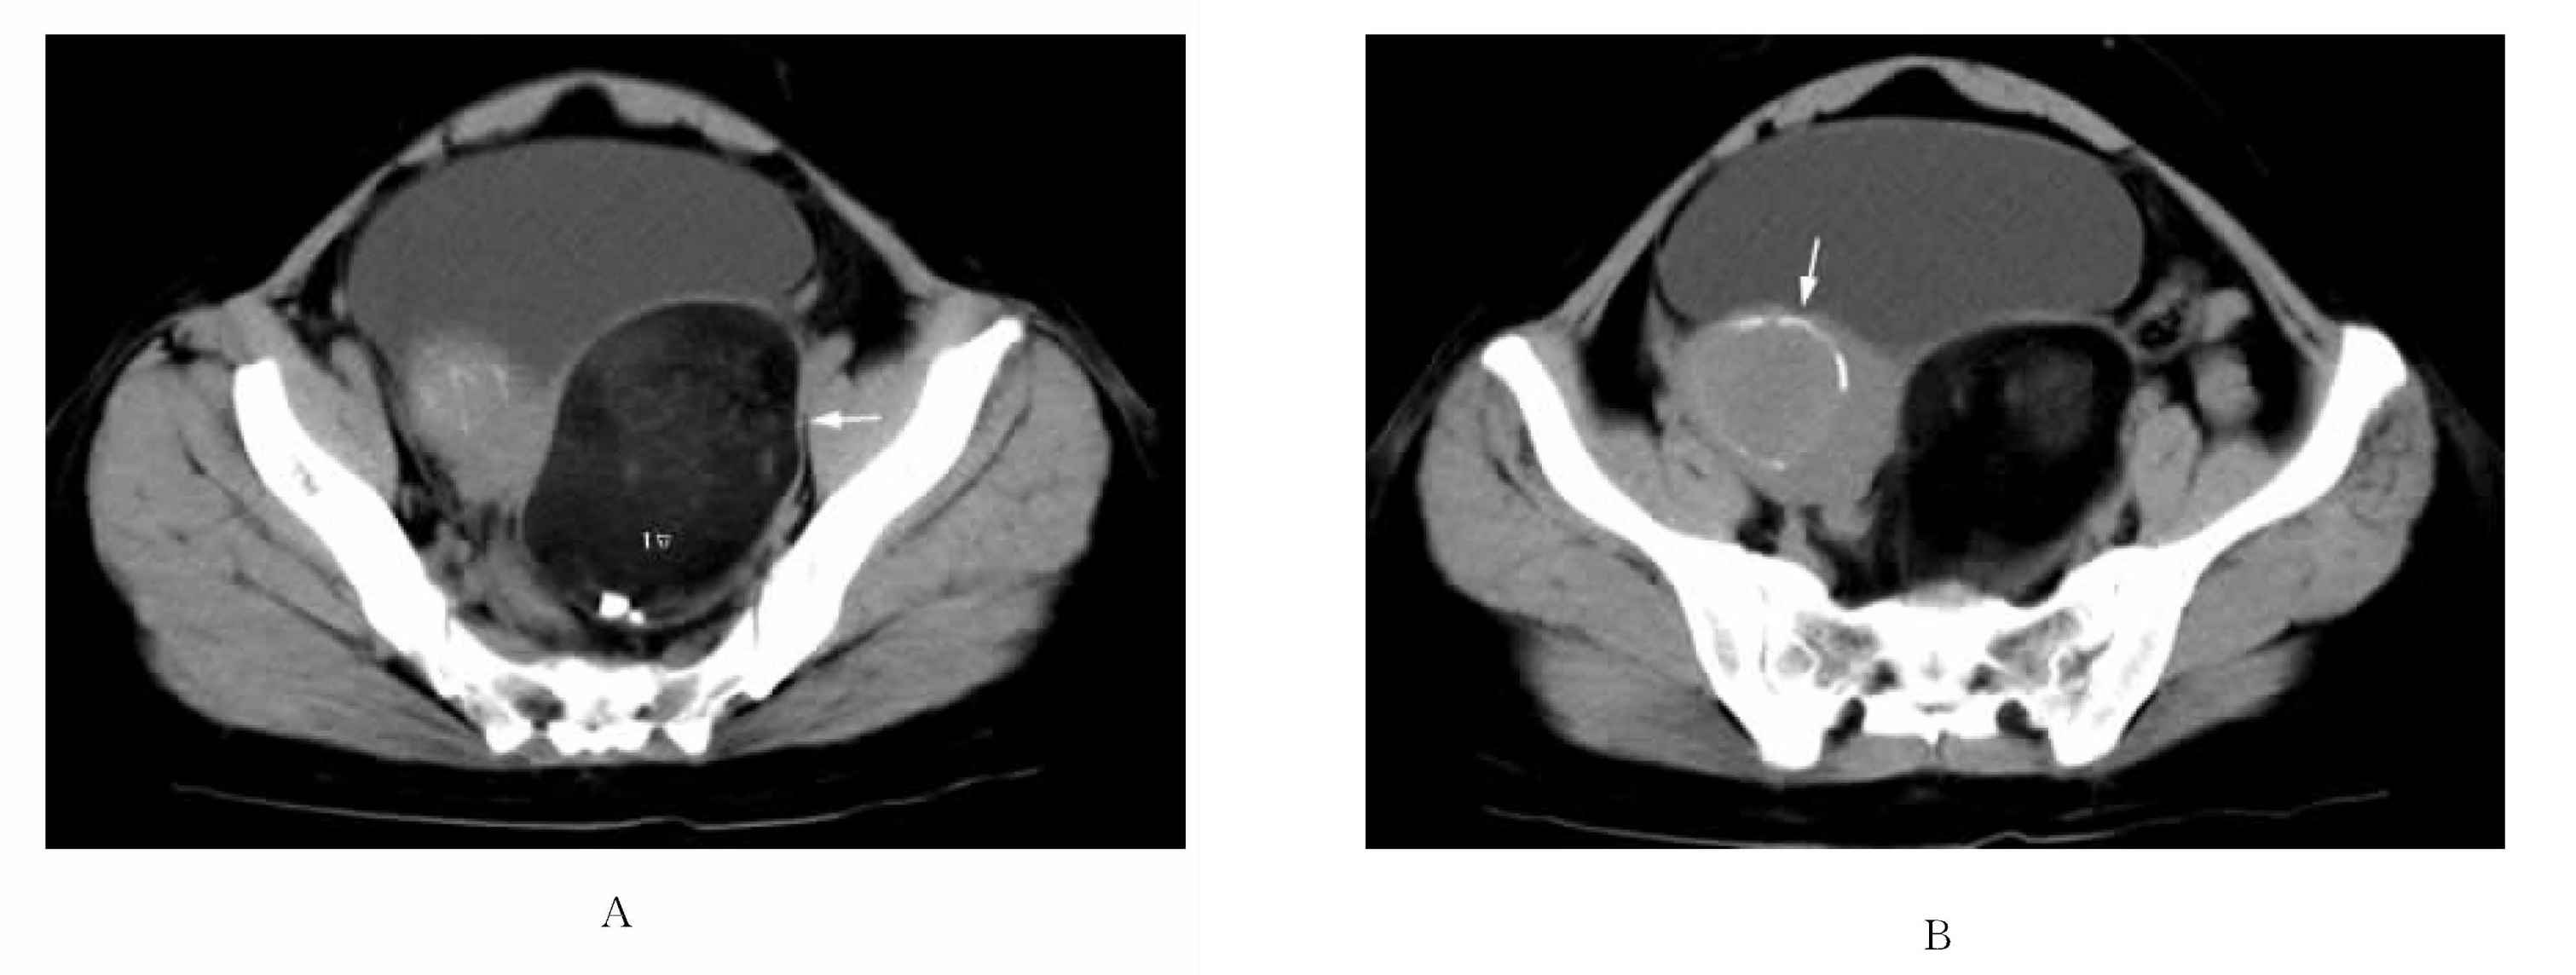
\includegraphics[width=.7\textwidth,height=\textheight,keepaspectratio]{./images/Image00411.jpg}
 \captionsetup{justification=centering}
 \caption{卵巢畸胎瘤\\{\small A、B为同一患者。子宫左上方有以脂肪密度为主的椭圆形肿块,其内有絮状高密度灶和牙齿状高密度灶;B图同时可见子宫内等密度的子宫肌瘤,边缘钙化}}
 \label{fig21-13}
  \end{figure} 

根据肿瘤内脂肪组织的含量,其CT表现可分为5型。①液性为主型:肿瘤主要为液性,含少量脂肪且常位于边缘。②液脂型:含相近数量的液体和脂肪。③头结节型:由脂肪成分和大小不等的头结节组成。④脂肪瘤型:由密度不均匀或均匀的脂肪组织构成。⑤囊肿型:完全由液性组织构成。

头结节是囊性畸胎瘤另一相对特异性征象,见于48%~80%的病例。结节通常为单个,亦可多个,直径一般为1.0~4.5cm大小;呈圆形或卵圆形,边缘清晰,与囊壁呈锐角相交;结节密度可为液性或软组织,常无强化。60%结节中见脂肪,45%见钙化或牙齿,65%可见源于结节的毛发。另外,头结节还是恶变的好发部位。

国外有学者认为直径>5cm的实性头结节,有明显强化并与囊壁呈钝角相交系恶变征象或提示为恶性囊性畸胎瘤。此外,约一半有钙化或牙齿,以单个点、片、线或结节状多见,大多位于头结上,其余在囊壁上。

2.未成熟畸胎瘤:多为实性,少数为囊性。常较大,呈分叶状,瘤内含散在不规则片状钙化及数量不等的脂肪,后者常提示诊断。瘤内亦可有出血和坏死。32%~58%的未成熟肿瘤易发生沿腹膜播散的种植转移。

3.卵巢甲状腺肿:呈分叶状、多房、厚分隔的囊实性肿块,可有环状、结节状钙化,实性区有明显强化,约50%合并成熟性畸胎瘤。

\subsection{卵巢纤维瘤}

本病为良性卵巢性索间质肿瘤,占所有卵巢肿瘤的2%~5%。

\textbf{【病理】}
本病是性索间质肿瘤中颗粒间质肿瘤的一个亚型,由卵巢间质细胞增生形成,其组织来源为卵巢间质或卵巢内非特异性纤维结缔组织。

常为单侧发病,右侧多见,仅4%~10%为双侧性。肿瘤中等大小,平均10cm左右,边缘光滑、质地硬(是质地最坚硬的卵巢肿瘤)。由成熟的纤维细胞和疏松的纤维结缔组织间质构成,呈束状彼此交叉排列,偶可恶变。

\textbf{【临床表现】}
多发生于40岁以上的中老年妇女,平均46岁。主要表现为下腹部肿块、疼痛以及肿块的压迫症状。因无内分泌功能,一般无月经紊乱。当合并腹水或胸腹水时称麦格斯(Meigs)综合征,肿瘤切除后胸、腹水可消失。 

\textbf{【CT表现】}
①盆腔内边界清楚的圆形或椭圆形肿块,常有分叶或不规则(图\ref{fig21-14})。②肿瘤多为实性,少数为囊性、囊实性,完全囊性者可见壁结节,实性部分与子宫等密度。③增强扫描常有轻度强化或几乎不强化。④50%可伴腹水,少数可伴大斑块钙化或出血、坏死囊变(呈囊实性)。

\begin{figure}[!htbp]
 \centering
 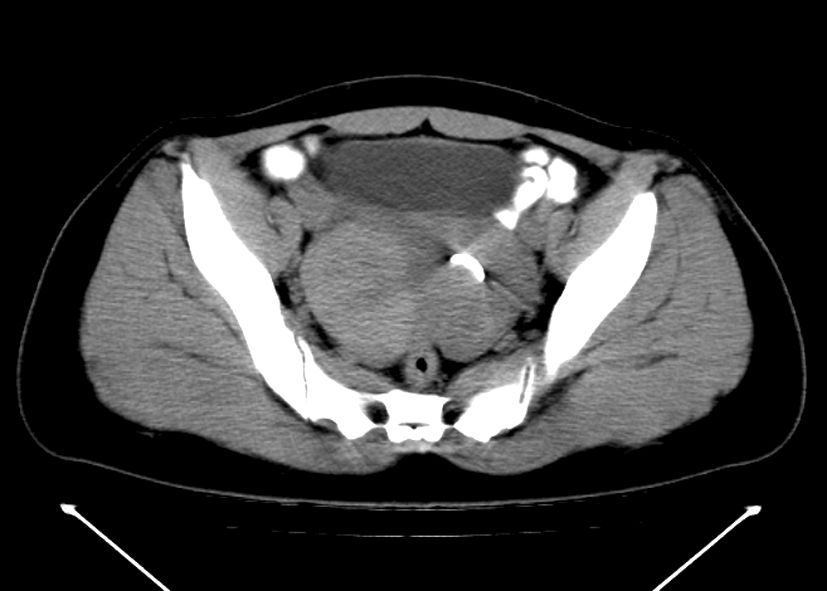
\includegraphics[width=.7\textwidth,height=\textheight,keepaspectratio]{./images/Image00412.jpg}
 \captionsetup{justification=centering}
 \caption{卵巢纤维瘤\\{\small 子宫右侧有椭圆形高密度肿块,密度欠均匀,边缘清晰锐利}}
 \label{fig21-14}
  \end{figure} 

本病需注意与子宫浆膜下肌瘤、阔韧带肌瘤及卵巢恶性肿瘤相鉴别,但常不易与恶性肿瘤鉴别。

\subsection{卵泡膜细胞瘤}

本病亦为卵巢性索间质肿瘤,少见,占全部卵巢肿瘤的0.5%~1.0%,约2%~5%为恶性。

\textbf{【病理】}
本病为来自卵巢性索间质的特殊间胚叶组织向卵泡膜细胞分化而形成的肿瘤,当其与颗粒细胞瘤共同存在时称为颗粒-卵泡膜细胞瘤。有些病例难以鉴别是纤维瘤还是卵泡膜细胞瘤,或者二者共同存在时,称为纤维-卵泡膜细胞瘤。

多为单侧发生,极少为双侧性。肿瘤大小不等,小者仅显微镜下可见,大者充满盆腹腔。常为圆形或卵圆形,也可呈分叶状。表面光滑,被覆薄的纤维包膜。常为实性,质地硬。

\textbf{【临床表现】}
更年期妇女多见,平均53岁,65%患者已经绝经。肿瘤增大可引起腹痛、腹胀和腹部包块等症状;肿瘤扭转可引起急腹症;少数可破裂或出血,也可有腹水或合并麦格综合征。可分泌雌激素,刺激子宫内膜增生、发生息肉,甚至腺癌,致子宫异常出血。

\textbf{【CT表现】}
无特异性。肿瘤多呈单侧圆形、卵圆形或不规则分叶状、实性或囊实性肿物,边缘光滑、清楚,少数可发生囊变、出血、坏死和钙化,肿瘤大小不一(图\ref{fig21-15})。我们还得见1例,大小约20cm×20cm×30cm,呈囊实性(囊性为主)。增强扫描呈轻度均匀或不均匀强化。虽然边界清楚,但常与恶性肿瘤难以鉴别,尤其囊实性者。

\begin{figure}[!htbp]
 \centering
 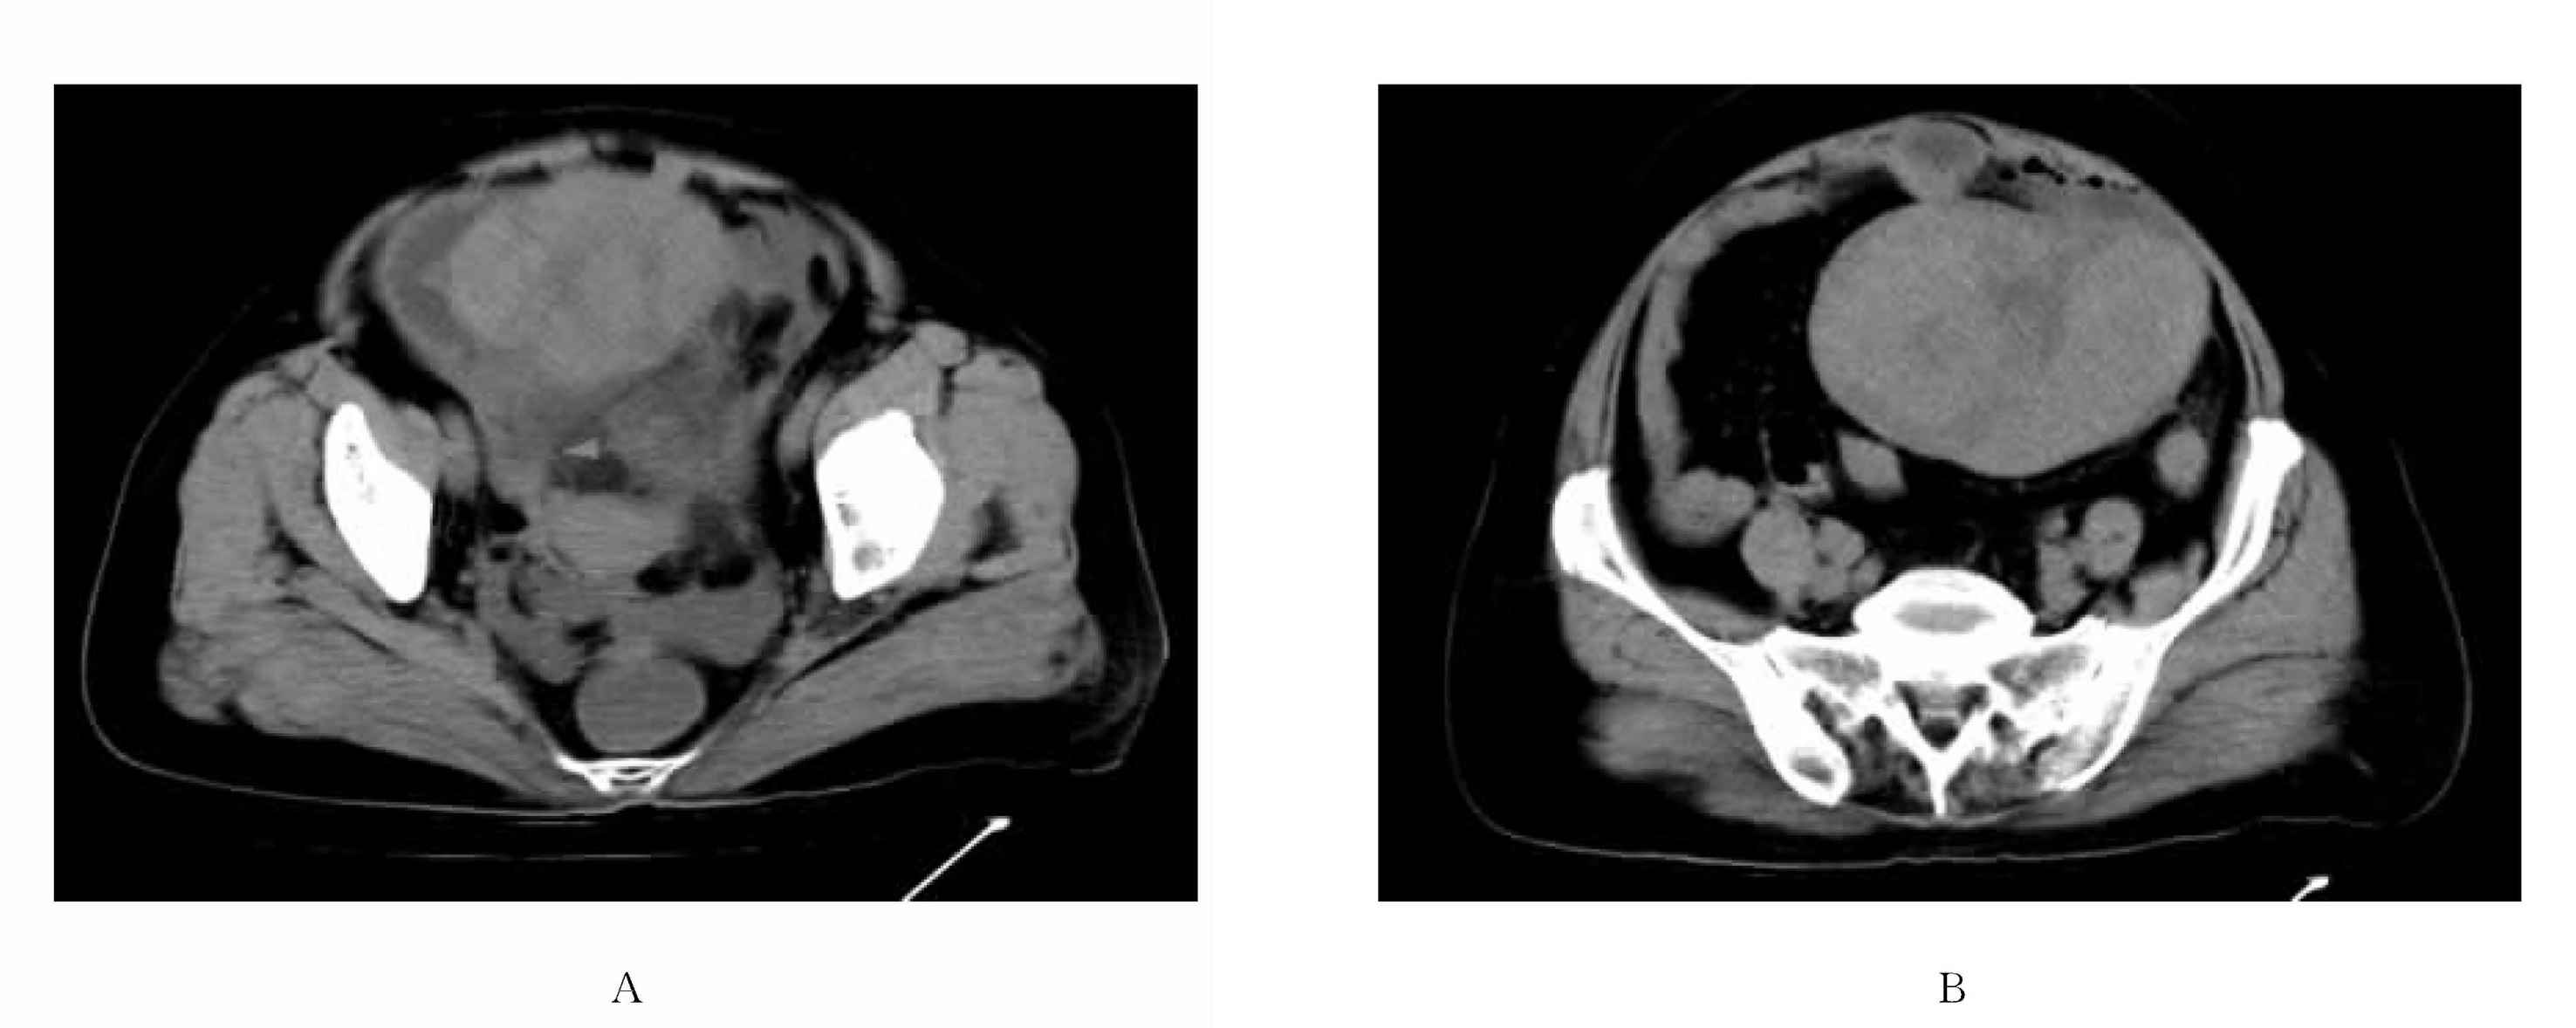
\includegraphics[width=.7\textwidth,height=\textheight,keepaspectratio]{./images/Image00413.jpg}
 \captionsetup{justification=centering}
 \caption{右侧卵巢卵泡膜细胞瘤\\{\small A、B为同一患者,可见囊实性肿块(实性为主),并可见盆腔积液(子宫直肠隐窝)。本例肿瘤有扭转,移向前方,子宫右侧可见扭转的蒂部}}
 \label{fig21-15}
  \end{figure} 

\subsection{卵巢浆液性和黏液性囊腺癌}

卵巢癌是最常见的恶性肿瘤,主要为浆液性囊腺癌和黏液性囊腺癌,而其他类型卵巢癌均少见。

\textbf{【病理】}

1.浆液性囊腺癌:占所有卵巢癌的50%以上,双侧者40%~60%,绝大多数由囊腺瘤恶变而来。肿瘤为囊实性,瘤内有许多大小不等的囊性区,内含陈旧性出血,囊壁上有明显的乳头状突起。

2.黏液性囊腺癌:占卵巢癌的15%~20%,双侧者不到10%。肿瘤为多房状,囊内有乳头状突起。

3.转移途径:包括局部侵犯、腹膜腔的直接种植和淋巴转移,而血行转移较为少见。在腹膜直接种植中,黏液性囊腺癌可形成腹腔假性黏液瘤。

\textbf{【临床表现】}
浆液性囊腺癌好发于40~70岁,黏液性囊腺癌好发于30~65岁。早期无特殊症状,晚期可有腹块及邻近脏器受压症状及消瘦、乏力、贫血等恶病质症状。

\textbf{【CT表现】}

1.浆液性囊腺癌:肿块约半数可>15cm,呈单房或多房的囊实性。囊壁厚薄不一,有乳头状突起或肿块,增强扫描强化显著。肿块内可见钙化。85%确诊时已有卵巢外播散、转移,淋巴转移等,如侵及输尿管可发生肾积水;侵及子宫可致子宫增大;侵及腹膜可形成腹膜结节、大网膜饼状增厚等。

2.黏液性囊腺癌:肿瘤巨大可达50cm,常为多房囊性或囊实性,极少数为实性。钙化少见。囊壁及间隔厚薄不一,有乳头状突起或肿块,强化也显著。确诊时也多有卵巢外播散、转移,淋巴转移等,还可有腹膜假性黏液瘤(图\ref{fig21-16})。

\begin{figure}[!htbp]
 \centering
 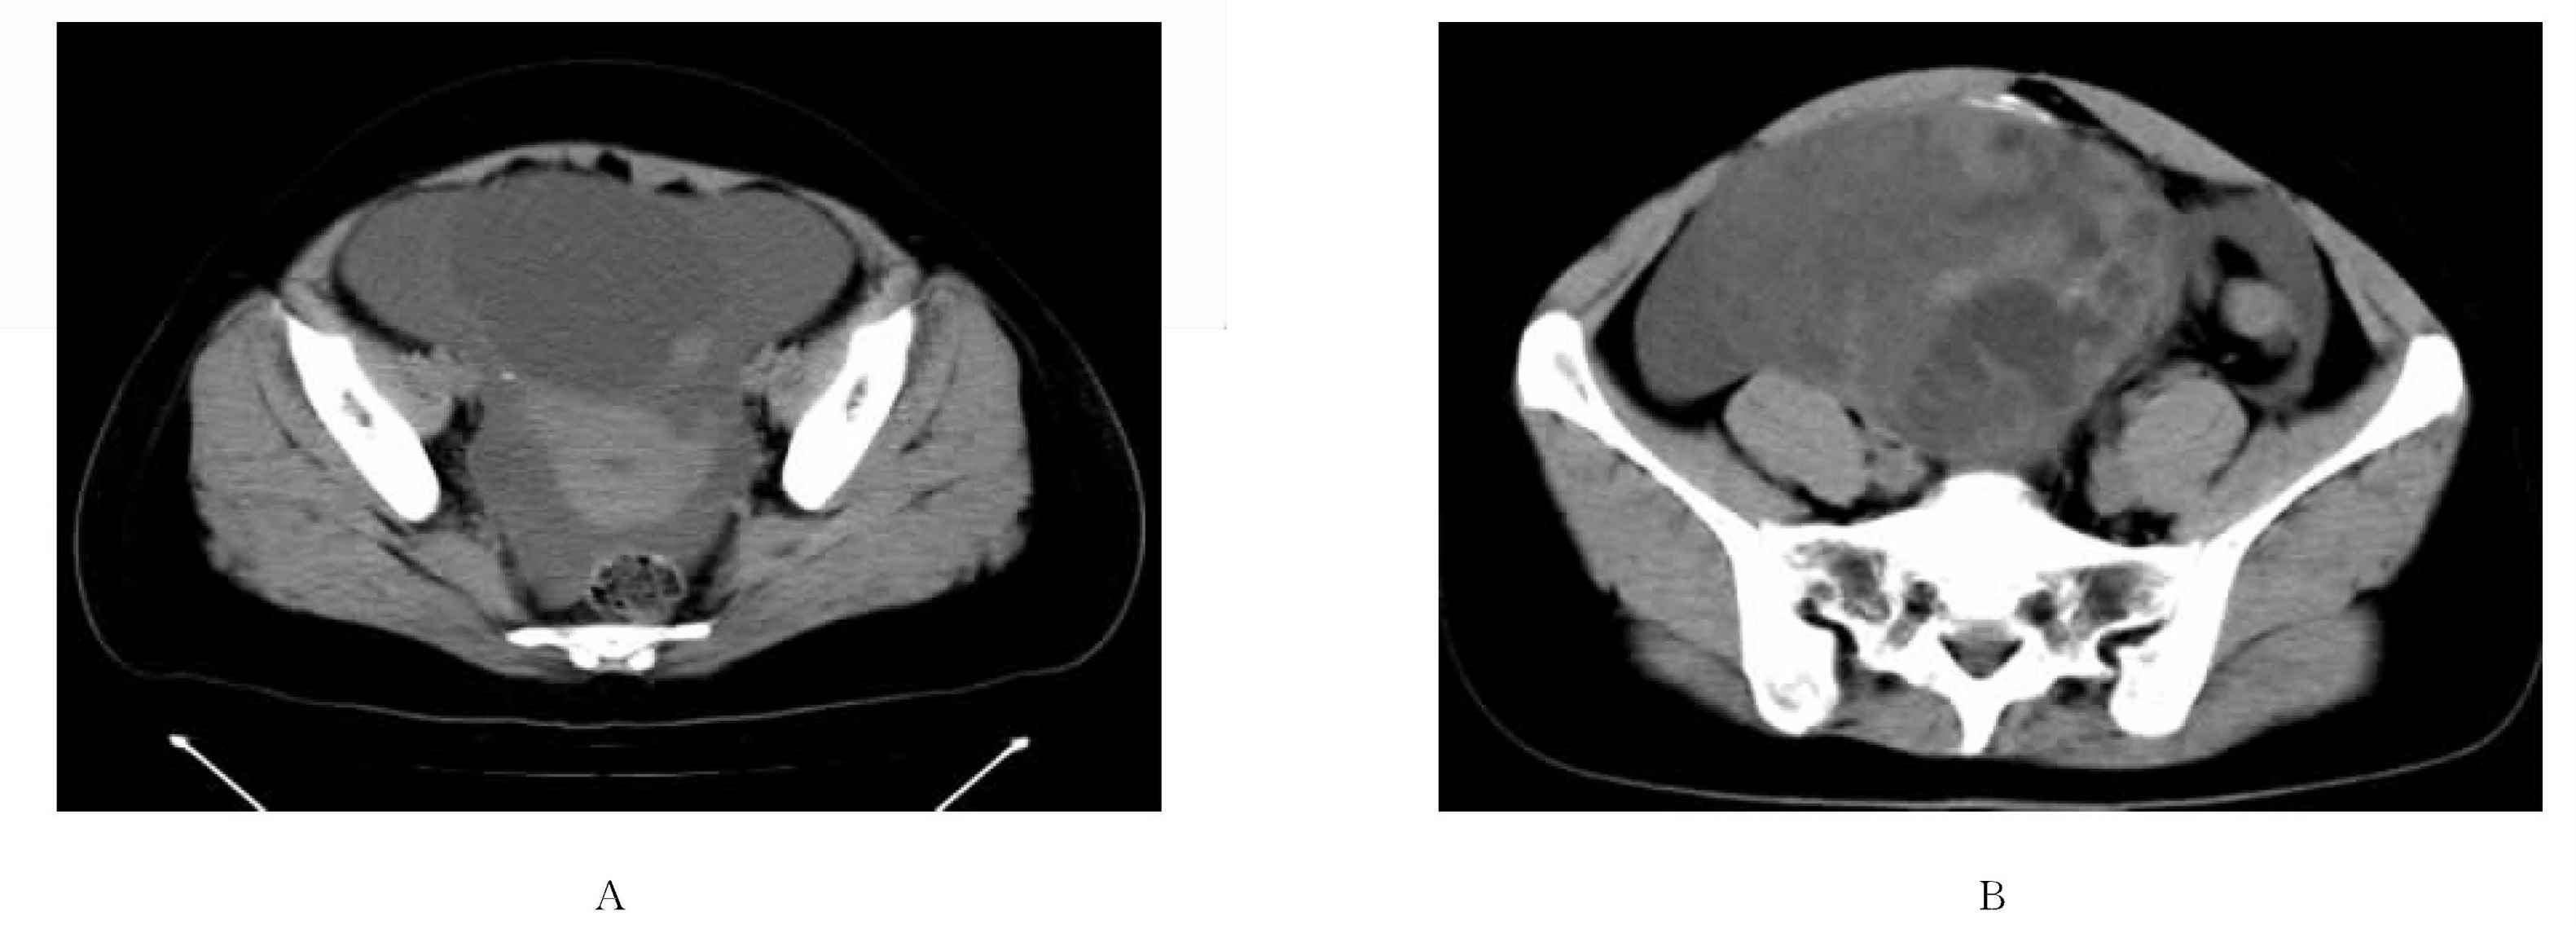
\includegraphics[width=.7\textwidth,height=\textheight,keepaspectratio]{./images/Image00414.jpg}
 \captionsetup{justification=centering}
 \caption{卵巢黏液性囊腺癌\\{\small A、B非同一患者。A示盆腔内巨大囊实性肿块,以囊性为主,可见一壁结节,伴盆腔积液(子宫直肠隐窝)。B示盆腔内巨大囊实性肿块,形态不规则,实性成分较多}}
 \label{fig21-16}
  \end{figure} 

\textbf{【鉴别诊断】}
卵巢恶性肿瘤以囊腺癌最常见,并有一定CT特征,其他如子宫内膜样癌、未分化癌、颗粒细胞瘤、无性细胞瘤、胚胎癌等则多为实性或囊实性肿块,其CT表现无特异性(见表\ref{tab21-2})。

\begin{table}[htbp]
\centering
\caption{几种主要卵巢恶性肿瘤的临床及CT特点}
\label{tab21-2}
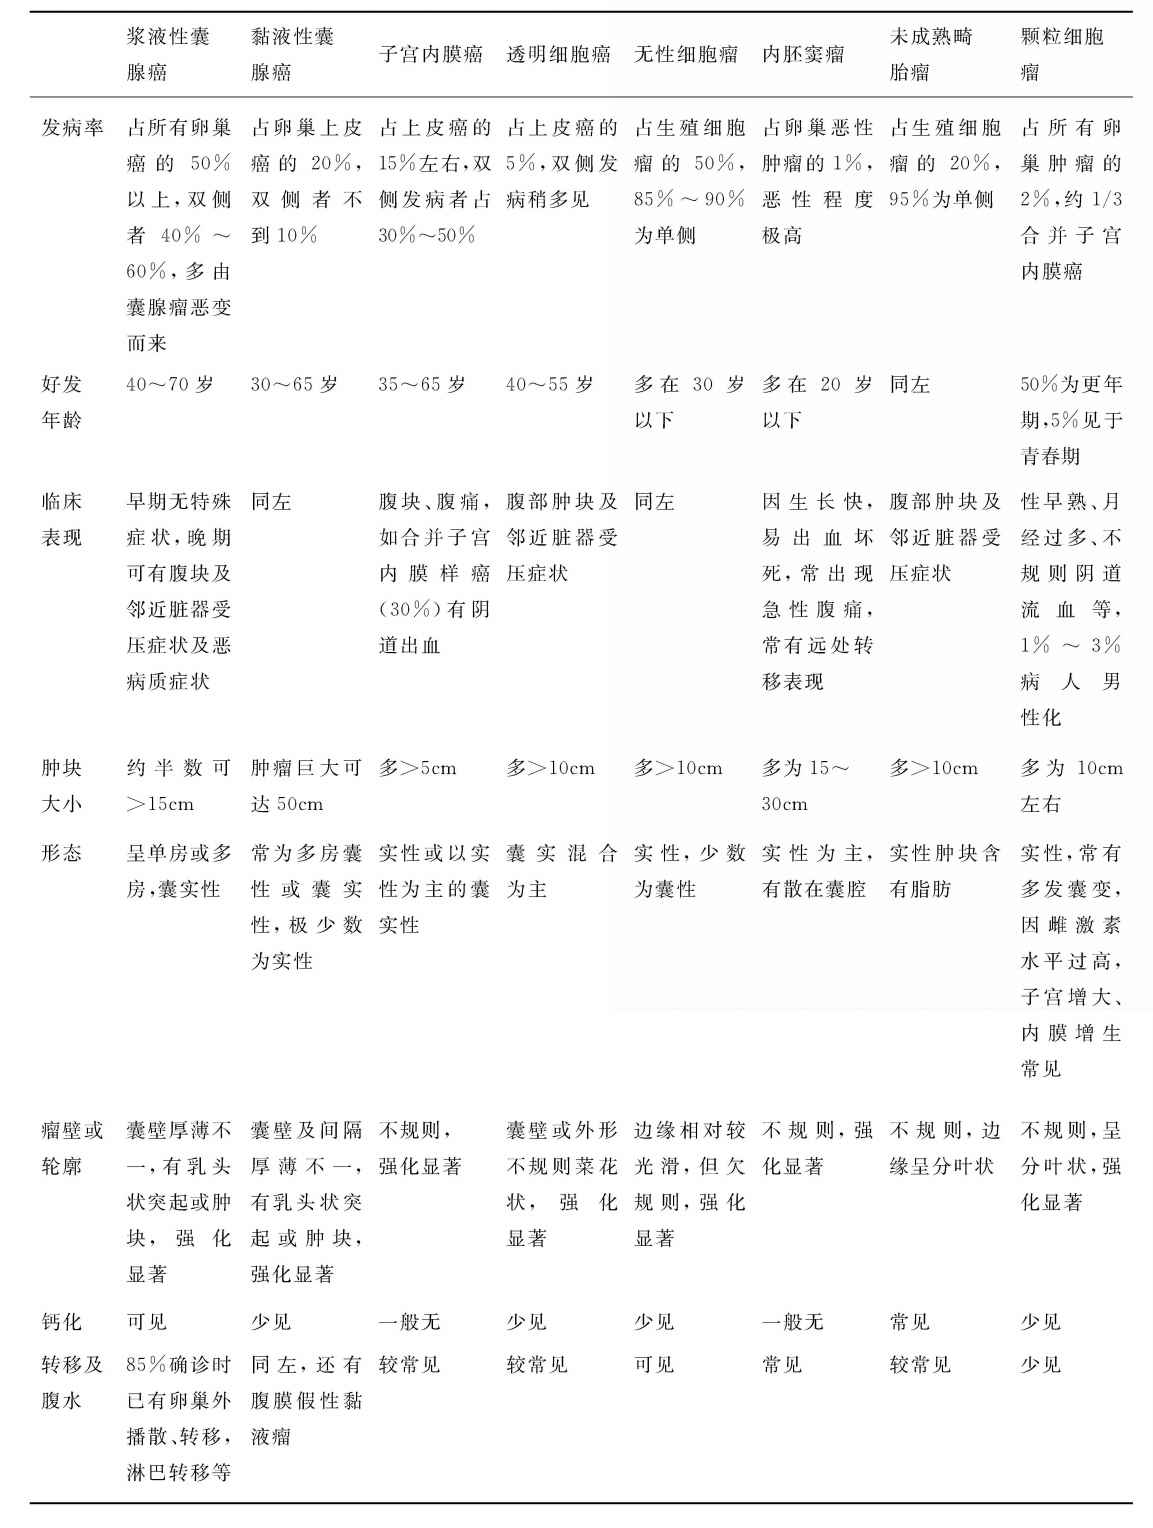
\includegraphics[width=\textwidth,height=\textheight,keepaspectratio]{./images/Image00415.jpg}
\end{table}

\subsection{卵巢转移瘤}

转移性卵巢癌的发病率为5%~10%,任何恶性肿瘤都可以转移至卵巢。

\textbf{【病因病理】}
在亚洲以胃肠道肿瘤尤其是胃癌最常见,在西方国家则以结肠癌最常见。次为乳腺癌。含有大量印戒细胞而间质来自卵巢的转移瘤称为克鲁根勃(Krnkenberg)瘤,占卵巢全部恶性肿瘤的4%~10%,它主要来自胃,但亦可来自乳腺、肠或其他含黏液腺的器官。转移瘤倾向于双侧卵巢发病。转移途径可为直接侵犯、经输卵管转移、淋巴转移或血行转移,主要经淋巴转移。

\textbf{【临床表现】}
多见于40~50岁。往往转移瘤症状较原发瘤更明显,表现为下腹部肿块,生长迅速,并有腹胀和腹痛,常出现腹水和(或)胸腔积液。

\textbf{【CT表现】}
转移瘤以实性为主或为混合性肿块,界限欠清。Krukenberg瘤一般为双侧肾形实性肿块。国外文献认为,大部分来源于胃、子宫内膜及乳腺者有大量的实性成分,而来源于结肠者则倾向于囊性为主或混合性。

\textbf{【鉴别诊断】}
转移瘤CT表现非常类似于原发性癌,尤其类似黏液性囊腺癌,不结合临床常难以鉴别。但对年轻的女性患者,盆腔出现双侧混合性或以实性为主的肿块,且伴消化道病史者,应想到转移瘤可能,并进一步检查。

\subsection{卵巢淋巴瘤}

\textbf{【病理】}
卵巢无淋巴细胞,故淋巴瘤是否可来源于卵巢尚有争论。但文献报道淋巴瘤可原发于卵巢。其中Burkitt淋巴瘤是一种少见的特殊类型的高度恶性B细胞淋巴瘤,由于Burkitt在非洲发现而得名,发病高峰在大龄儿童,肿块常位于回盲部、腹膜后、卵巢、肾或乳腺。

\textbf{【CT表现】}
卵巢淋巴瘤常发病于一侧,偶为双侧。卵巢明显增大,或由多个软组织肿块融合而成,呈软组织密度,其内无脂肪、钙化及囊变。增强扫描可有轻度强化。肿块较大时可有邻近脏器如子宫和膀胱等受压表现。大的肿块不易判断其来源。

\subsection{小结}

\subsubsection{卵巢肿瘤的影像学分型}

可分为以下3型。Ⅰ型:为囊性。Ⅱ型:为囊实性,其中又分为3个亚型。Ⅱa型以囊为主(囊性成分>2/3);Ⅱb型为混合性(实性成分占1/3~2/3);Ⅱc型以实性成分为主(实性成分>2/3)。Ⅲ型:为实性。Ⅰ、Ⅱa型有单房或多房之分。

在分析肿瘤的囊壁与囊内间隔厚度时以3mm为界,<3mm为薄壁;>3mm为厚壁,并有规则与不规则之分。部分Ⅱ型者可出现囊内壁结节和(或)伴有不规则软组织成分,亦可有囊外壁结节。

良性囊腺瘤以Ⅰ型常见,恶性囊腺肿瘤以Ⅱa、Ⅱb型常见。转移瘤以Ⅱ型最常见,其次为Ⅲ型,Ⅰ型少见。其他恶性肿瘤亦以Ⅱ、Ⅲ型常见。

\subsubsection{卵巢恶性肿瘤的CT特征和腹膜种植的常见部位}

不同组织类型的卵巢恶性肿瘤其CT特征不同。①病灶可为单侧性或双侧性,但以双侧性多见。②肿瘤轮廓多数不规则,呈分叶状边缘,且常侵犯周围脏器。③病灶多呈囊、实混合性。囊性灶其囊壁和间隔厚薄不一(多>3mm),囊腔内壁凹凸不平或出现壁结节。实性灶常呈斑片或菜花状肿块突向囊壁内外。④少数病灶有钙化(约26%)。⑤病灶实性部分有强化,增强值常在25Hu以上。⑥病程短而病变范围较广,常在发现病灶的同时已有腹膜扩散种植(76%),而淋巴和血行转移较少(10%及5%)。腹膜转移灶也可有钙化表现。⑦可有胸、腹水表现。

腹膜种植是卵巢恶性肿瘤的主要播散途径,可累及所有腹膜面。种植的部位主要包括:腹膜凹陷处(子宫直肠窝、肝肾隐窝、右结肠旁沟)、膈下间隙、肝表面、肝门、肝裂、脾表面、网膜和肠系膜。国外有学者报道最常见部位是右膈下间隙(与呼气时膈下形成负压有关),其次为大网膜和子宫直肠陷凹。

\subsubsection{卵巢良恶性肿瘤的鉴别要点及与炎症的鉴别}

良恶性肿瘤的鉴别要点为:①良性肿瘤轮廓光滑,多为均一单房或多房水样密度肿块,囊壁及间隔均匀,厚度<3cm;虽可有乳头状软组织突起,但软组织成分相对较少,增强扫描无明显强化。②恶性肿瘤多为囊实性肿块或实性肿块伴有一定的坏死囊变,轮廓不光整,壁厚而不规则,增强扫描实性部分和壁多明显强化;病变范围多数广泛,常合并腹水和盆腔淋巴结增大。钙化无特异性,良恶性肿瘤均可见及。

但少数病例良、恶性不易鉴别,如纤维瘤、转移瘤、良性肿瘤小区恶变(如囊腺瘤)及交界性肿瘤,需病理组织学定性。而且良性病变也可出现较明显的实性肿块和壁结节,恶性病变有时壁结节不明显且囊壁较光滑、厚薄较均匀。

此外,输卵管、卵巢的急慢性炎症所致炎块和伴脓肿形成时,病灶边缘模糊不规则;增强扫描强化明显,易误诊为卵巢癌。但病灶内有气体时强烈提示脓肿形成。结合临床进行鉴别甚为重要。

\subsubsection{卵巢肿瘤与子宫肿瘤的鉴别}

两者应从以下3方面鉴别:①病灶与子宫的接触面是锐角还是钝角,即一般卵巢病灶与子宫呈锐角相交,而子宫肿瘤则与子宫呈钝角相交,不易分开。②病灶增强是否与子宫一致,子宫肿瘤多与子宫强化一致。③是否伴有腹水、网膜腹膜转移,除非子宫肿瘤巨大,一般不引起腹水,且网膜腹膜转移少。

但有时卵巢肿瘤与子宫浆膜下肌瘤可鉴别困难,亦可与下腹部肠道肿瘤、肠系膜肿瘤及腹膜后肿瘤难以鉴别。盆腔肿块的双侧性,有利于卵巢肿瘤的定位诊断。

\subsubsection{卵巢囊性病变的CT分析}

1.卵巢囊性病变可见于单纯囊肿、功能性囊肿、囊腺瘤、囊腺癌、囊性畸胎瘤、子宫内膜异位症、Krukenberg瘤、中肾管囊肿、陈旧性异位妊娠、卵巢脓肿及输卵管脓肿、炎症积水等。

2.CT在分析时应注意病变的位置、大小、形态、轮廓、密度、囊壁软组织成分多少,以及有无脂肪灶、钙化骨化和邻近直接浸润、种植、淋巴及血行转移、腹水等。

3.良性囊性病变常为圆形或椭圆形,囊壁及间隔薄而规则,厚度<3mm。

4.恶性病变多为双侧,形态不规则,囊壁及分隔厚(>3mm)呈不规则结节状,边缘模糊且强化明显。

5.钙化对良、恶性病变的鉴别无意义,但与脂肪成分并存有助于畸胎瘤的诊断。

\section{输卵管病变}

\subsection{输卵管积水}

\textbf{【病因病理】}
本病是由于输卵管伞端闭塞,继发液体聚集或出血性分泌而致。原因较多,最常见为输卵管炎或由于以往手术、子宫内膜异位引起粘连或输卵管肿瘤引起阻塞而致。

\textbf{【影像学表现】} 呈薄壁囊状水样低密度灶,无特异性。

\subsection{输卵管肿瘤}

原发性输卵管肿瘤罕见,约占所有妇科肿瘤的0.3%,最常见为腺癌。

\textbf{【临床表现】}
多见于产次少的妇女或未生育妇女,平均年龄为55岁。常有阴道流血和分泌物增多、盆腔肿块或疼痛。

\textbf{【影像学表现】}
难与卵巢肿瘤鉴别。①呈实性或囊实性附件区肿块,亦可难以显示。②约10%~15%为双侧性。③局部可累及卵巢、子宫、乙状结肠和其他盆腔内结构。④经管腔可致腹膜腔播散;淋巴转移率高,可转移到主动脉旁和髂组淋巴结。

\subsection{输卵管妊娠}

受精卵在子宫腔以外的部位种植发育者称为异位妊娠,又称子宫外孕。有输卵管妊娠、卵巢妊娠、腹腔妊娠、宫颈妊娠,约95%为输卵管妊娠。

\textbf{【病因】}
任何妨碍受精卵进入子宫腔的因素均可造成输卵管妊娠,慢性输卵管炎是其主要原因。此外,输卵管发育异常(如过长、过细、肌肉发育不良)、输卵管结扎后再通、输卵管子宫内膜异位症、盆腔肿瘤的压迫或牵引等均可可致受精卵的运行受阻或输送延迟,不能按时进入子宫,而在输卵管某个部位着床。

\textbf{【临床表现】}
输卵管妊娠流产或破裂前,往往症状及体征不明显,诊断比较困难,有时仅为停经后下腹隐痛或憋胀感。

临床所见多为破裂时或破裂后的症状。①腹痛:为其主要症状,患者突感下腹一侧撕裂样疼痛或阵发性绞痛;②阴道流血:为不规则点滴状,量少色褐红,也有无阴道流血者;③停经史;④休克;⑤腹部检查:腹部压痛、反跳痛,有时可摸到下腹部压痛的肿块等;⑥尿妊娠试验呈阳性或弱阳性。

\textbf{【CT表现】}

1.根据其CT特点可分为以下5类。①孕囊型:发现完整的妊娠囊样结构;②囊肿型:主要表现为囊性包块;③包块型:主要呈混杂密度肿块,部分可见变形的妊娠囊样结构;④陈旧包块型:也呈混杂密度块,周围有弧形钙化;⑤出血型:子宫旁大片状或不规则出血灶。其中以包块型最常见,其次为囊肿型和孕囊型。

2.直接征象:附件区发现完整或变形的妊娠囊。①包块软组织部分密度不均,显著强化;②孕囊约呈>1cm的近水样低密度灶,囊壁显著强化。

3.间接征象:①附件区囊性包块(可达5cm左右)中有强化的异常密度灶;②附件区混杂密度包块,以实性成分为主,增强呈轻中度不均匀强化;③盆腔内宫旁大片稍高密度影,无明显强化;④子宫直肠隐窝内见血性密度影。

4.陈旧性输卵管妊娠的特点:由于输卵管妊娠反复出血、新旧并存,流动后凝固,无血供及良性无侵犯的病理特点。其CT表现有以下特点:①盆腔内混杂密度肿块:平扫呈圆形或卵圆形,有时可见假包膜,巨大肿块有时可包绕子宫,但无侵犯征象。其内密度不均,以较高密度(CT值45~80Hu)为主,其间夹杂低密度区。增强扫描肿块无强化或轻度不均匀强化。②子宫直肠陷凹积液:有时其内可见高密度影呈液-液平面表现,可能在陈旧性积血的基础上又有新的出血。③大网膜聚集现象:由于输卵管妊娠流产或破裂后被大网膜包绕所致。

有学者认为,当发现宫旁有不规则软组织包块,界限不清,其内有新鲜出血所致的高密度灶,且增强后仅见包膜强化而内部不强化者,可以认为是陈旧性异位妊娠的特征性CT表现。

\textbf{【鉴别诊断】}

1.出血性输卵管炎:其症状、体征与异位妊娠相似,但前者一般无肿块形成。

2.原发性输卵管及卵巢的恶性肿瘤:发生囊变坏死时,也可呈高、低密度相间的肿块,但其软组织成分较多,多呈分叶状,增强扫描明显强化。如有转移则可进一步确诊。

3.卵巢良性肿瘤:多为囊性包块,壁光滑清晰,其内一般不伴高密度灶。

4.子宫体癌:子宫呈分叶状增大,宫腔变形,肌层局限性增厚,其内有低密度区。

5.阑尾周围脓肿:无闭经史,有转移性右下腹疼痛史,全身感染中毒症状明显。

\section{盆腔其他病变}

\subsection{盆腔脂肪增多症}

本病是一种大量脂肪组织非正常堆积于盆腔内,造成对盆腔内脏器包绕、压迫、推移和牵拉。

\textbf{【病因病理】}
本病可能与脂肪代谢、内分泌紊乱、过度肥胖造成的过度堆积有关。脂肪沉积以直肠、膀胱周围为著,从而造成直肠、下段输尿管、后尿道等一系列梗阻改变,往往并发腹腔及腹膜后脂肪增多。

\textbf{【临床表现】}
大多见于30~50岁,男女之比为28∶1。主诉以泌尿系感染症状为主,其次是下消化道症状,年老患者可并存前列腺增生而产生相应症状。

\textbf{【CT表现】}
盆腔内呈均匀低密度,CT值在-100Hu左右。直肠、乙状结肠、膀胱、前列腺等受压移位和变形。总之,如显示盆腔多量脂肪和部分脏器受压变形可以明确诊断。

\subsection{盆腔静脉淤血综合征}

也有学者称为盆腔充血综合征。本病由Aran于1858年首先报道,是由于盆腔静脉曲张淤血引起的一种妇科疾病。

\textbf{【病因】}
不十分清楚。多认为可能是卵巢静脉功能不良(卵巢静脉的扩张和血液返流)所致。本病主要发生于育龄妇女,尤其是多产妇,可能与妊娠期间血容量生理性增加(因为妊娠时盆腔血容量会增加60倍,并且会持续到产后6个月)有关。但还有其他因素,如子宫位置异常,造成盆腔静脉扭结、淤血;雌激素、精神因素作为病因也有报道。

\textbf{【临床表现】}
其临床特性是不同程度的下腹部疼痛,并且持续6个月以上。在腹部压力突然增加,如行走、弯腰、搬动重物时出现下腹部疼痛,通常疼痛是单侧的。本病的一个显著特征是几乎全部发生于育龄期妇女。其他的表现还有骶部疼痛、痛经、性交痛、脐周痛、急性外阴部及下肢静脉曲张。泌尿系统症状主要有尿急,还可出现尿频、尿痛。常有情绪不稳定。临床检查可有卵巢点压痛和腹部触痛。

\textbf{【CT表现】}
CT检查应在深吸气下(增加腹部静脉压),延迟30秒和70秒行动脉期和静脉期盆腔扫描。CT的诊断依据是扩张的、显著强化的卵巢静脉包绕子宫和卵巢,如静脉直径>5mm即有诊断价值。

正常情况下,动脉期仅有动脉系统和肾静脉显影,卵巢静脉不显影,如其提前显影,与肾静脉同时出现,说明卵巢静脉功能不全,其内有返流存在。卵巢静脉显影后,子宫静脉和宫旁静脉也显影。

\subsection{骶尾部畸胎瘤}

盆腔内非脏器起源的畸胎瘤好发于骶骨前区域,而且儿童骶前间隙最常见的肿瘤是骶尾部畸胎瘤,多为良性。

\textbf{【病理】}
骶尾部畸胎瘤根据其体内外肿瘤的相对大小分为4型。Ⅰ型:体外为主型(47%);Ⅱ型:体外盆内型(34%);Ⅲ型:体外腹内型(9%);Ⅳ型:单纯骶前型(10%)。

组织学表现与其他部位者一致。良性(或成熟性)由分化好的外、中、内胚层来源的组织构成,其中皮样囊肿外层为纤维组织,内层为皮肤构成(含有皮肤附件)。恶性(或未成熟性)以实性为主,伴有囊性区,由来自3个胚层的成熟或未成熟组织构成。

\textbf{【临床表现】}
如果肿瘤较小仅限于骶前则不易发现,往往于成年后出现症状和体检而发现。可有骶尾部或下腹部疼痛不适,也可有便秘、尿频、尿急等症状。可触及包块。

\textbf{【CT表现】}
①多数良性畸胎瘤含有脂肪、钙化或骨化、囊性低密度区及软组织成分而具有特征性,邻近脏器可受推压。皮样囊肿有时可呈均匀的、囊状水样低密度,亦可因富含蛋白等原因呈均匀的圆形或类圆形高密度灶。②恶性畸胎瘤软组织成分所占比例大,也有脂肪和钙化、骨化成分,常破坏骶骨或侵犯邻近脏器,与其他恶性病变较难鉴别。③50%患者合并其他脊髓异常,隐性骶裂最常见,其次为脊髓纵裂或分节畸性。

\subsection{骶尾骨脊索瘤}

本病为一种少见的低度恶性肿瘤,很少转移,可侵入盆腔累及直肠、膀胱及子宫等。

\textbf{【临床表现】}
好发于40~70岁,男女之比约2∶1。多有骶尾部疼痛,可向下肢放射,亦可出现大小便次数及性状的改变。直肠指诊多可触及直肠后方肿块。

\textbf{【CT表现】}
病灶常位于骶尾交界处,呈溶骨性膨胀性骨质破坏表现。穿破骨皮质向盆腔内突起形成软组织肿块,肿块内可有残余碎骨块和不规则钙化表现(图\ref{fig21-17})。肿块常推移或侵犯邻近器官,并向外侵犯臀部肌肉,突向体表。

\begin{figure}[!htbp]
 \centering
 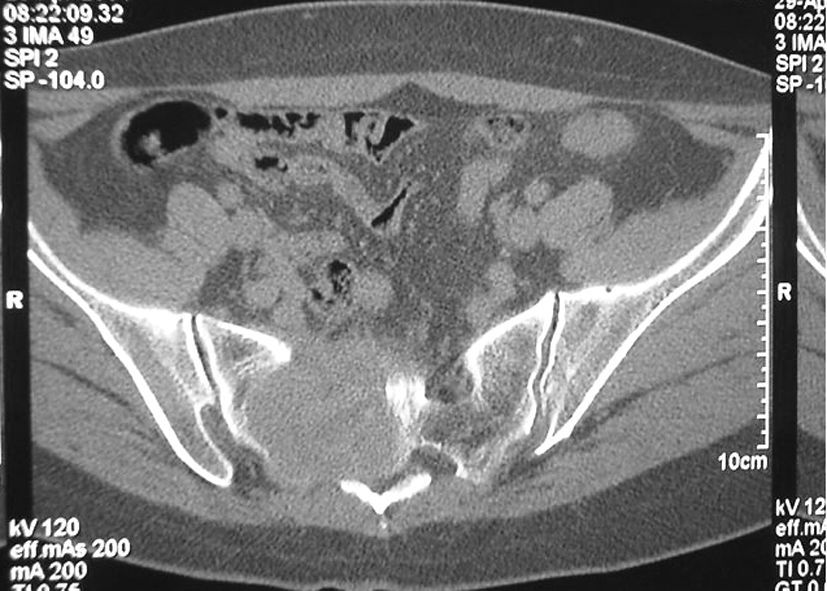
\includegraphics[width=.7\textwidth,height=\textheight,keepaspectratio]{./images/Image00416.jpg}
 \captionsetup{justification=centering}
 \caption{骶骨脊索瘤\\{\small 骶骨有溶骨性膨胀性骨质破坏,局部有软组织肿块}}
 \label{fig21-17}
  \end{figure} 

\subsection{盆腔器官外软组织肿瘤}

\textbf{【病理】}
该类肿瘤是指位于盆腔内,起源于腹膜外、腹膜及腹膜内器官间隙的软组织肿瘤,转移性和骨组织起源的肿瘤不包括在内。起源于腹膜外的肿瘤最多见,常见的有间叶源性肿瘤(平滑肌肉瘤、脂肪和脉管性肿瘤、纤维肉瘤等),其次是神经源性肿瘤(神经纤维肉瘤、神经纤维瘤和神经鞘瘤等)、胚胎残余源性肿瘤(囊性畸胎瘤、脐尿管囊肿等)。源于腹膜的肿瘤如腹膜间皮瘤极为少见。

\textbf{【临床表现】}
以下腹部疼痛不适和触及包块为主要表现。少数有便秘、尿频、尿急、血尿等症状。

\textbf{【影像学表现】}
①囊性肿块:一般为良性,主要有囊性畸胎瘤、脐尿管囊肿、囊性淋巴管瘤等。②囊实性或实性肿块:多为恶性,以平滑肌肉瘤和神经纤维肉瘤较多见,其他还有纤维肉瘤、脂肪肉瘤、血管源性肉瘤。良性的脂肪瘤、平滑肌瘤、神经纤维瘤等亦可呈囊实性或实性肿块,但包膜完整、界限清晰,无邻近浸润及其他转移表现。

\protect\hypertarget{text00029.html}{}{}

